\chapter{Applied Regression Modeling}

Regression modeling is a foundational technique in bioinformatics. However,  implementation of regression models in software produces a lot of output, and it's not always clear (a) what the model is saying about the data and the research question, (b) whether these results are due to a real discovery or a statistical artifact. In this workshop, we'll tackle both of these issues.

\textbf{Remember that the overarching goal of any modeling project is to learn something about your data that is actually true.}

\paragraph{Question 1} What is the gold standard for telling whether a model is capturing a true relationship in the data?

\vspace{30mm}

\paragraph{Question 2} What are the three main reasons for building a regression model?

\vspace{30mm}

\paragraph{Question 3} What are the formal assumptions of linear regression models? Which of these also apply to logistic regression models?

\newpage

%%%%%%%%%%%%%%%%%%%%%%%%%%%%%%%%%%%%%%%%%%%%%%%%%%%%%%%%%%%%%%%%%%%%%%%%%%%%%%%%

\section{Interpreting Linear Regression Models}

A linear regression model looks like this (also see Appendix):
$$ y = \beta_0 + \beta_1 x_1 + \dots + \beta_p x_p + \varepsilon $$
where we assume that the error, $\varepsilon$, is normally distributed, $\mathcal{N}(0, \sigma)$. Here is an example of a dataset that looks like it might adhere to such a model:

\begin{center}
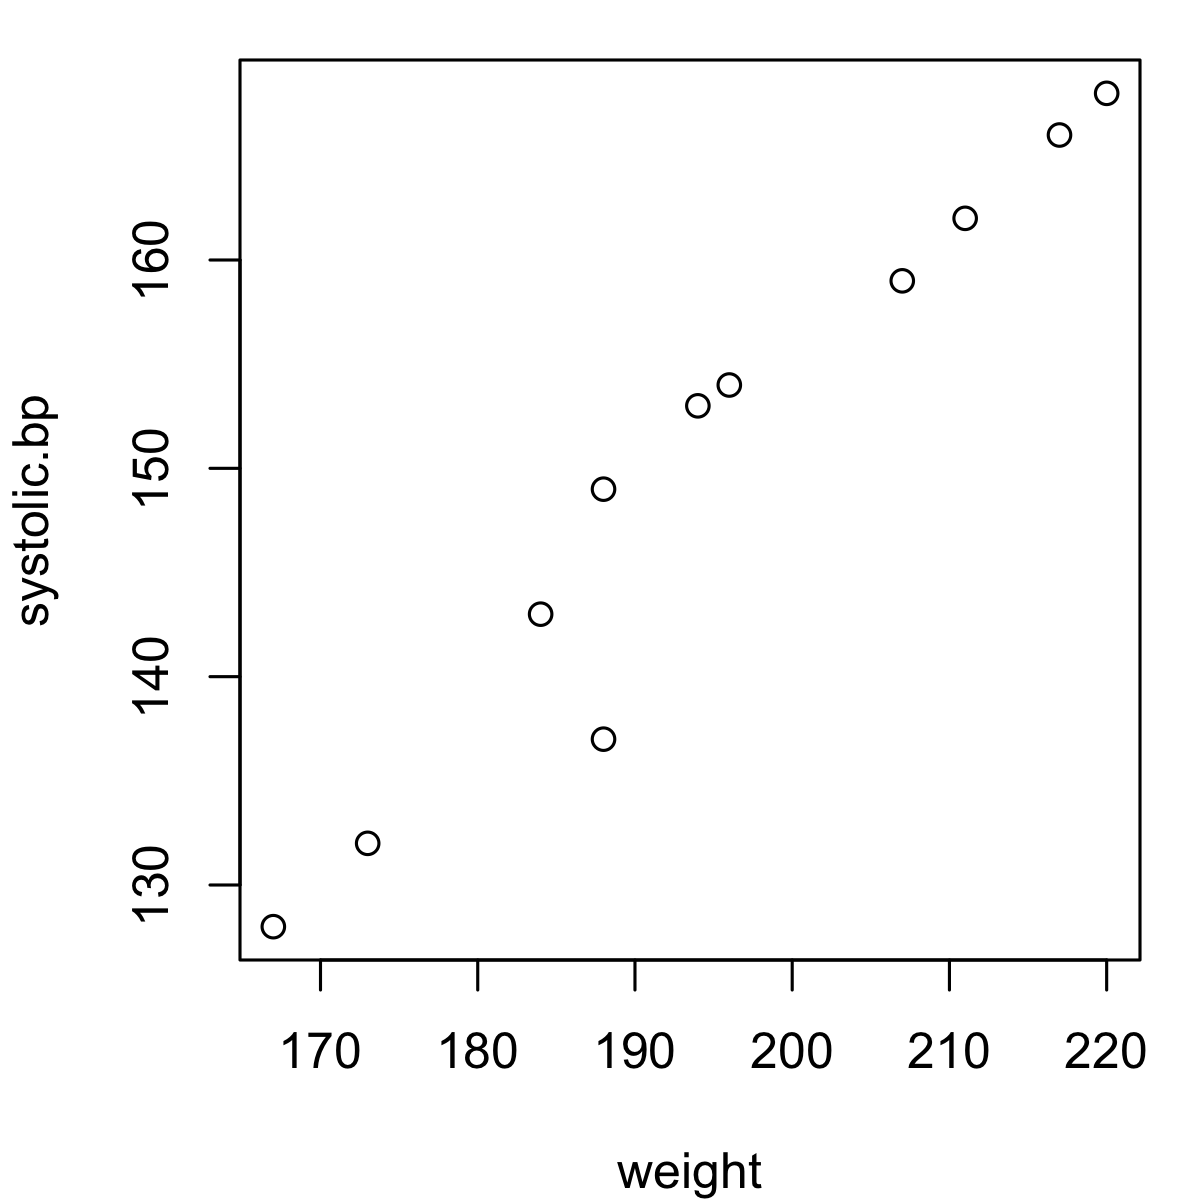
\includegraphics[width=0.4\textwidth]{img/systolic-bp-simple-plot.png}
\end{center}

\paragraph{Question 4} What are $n$ (the number of samples) and $p$ (the number of predictors) for this dataset?

\vspace{5mm}

Here is what happens when we fit a linear regression model to these data in R:
\begin{center}
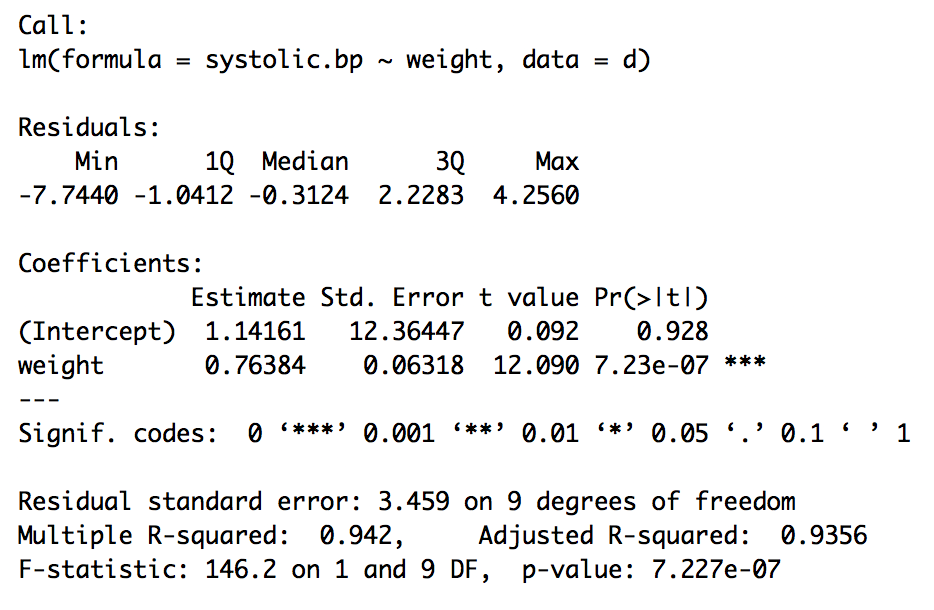
\includegraphics[width=0.6\textwidth]{img/systolic-bp-simple-model.png}
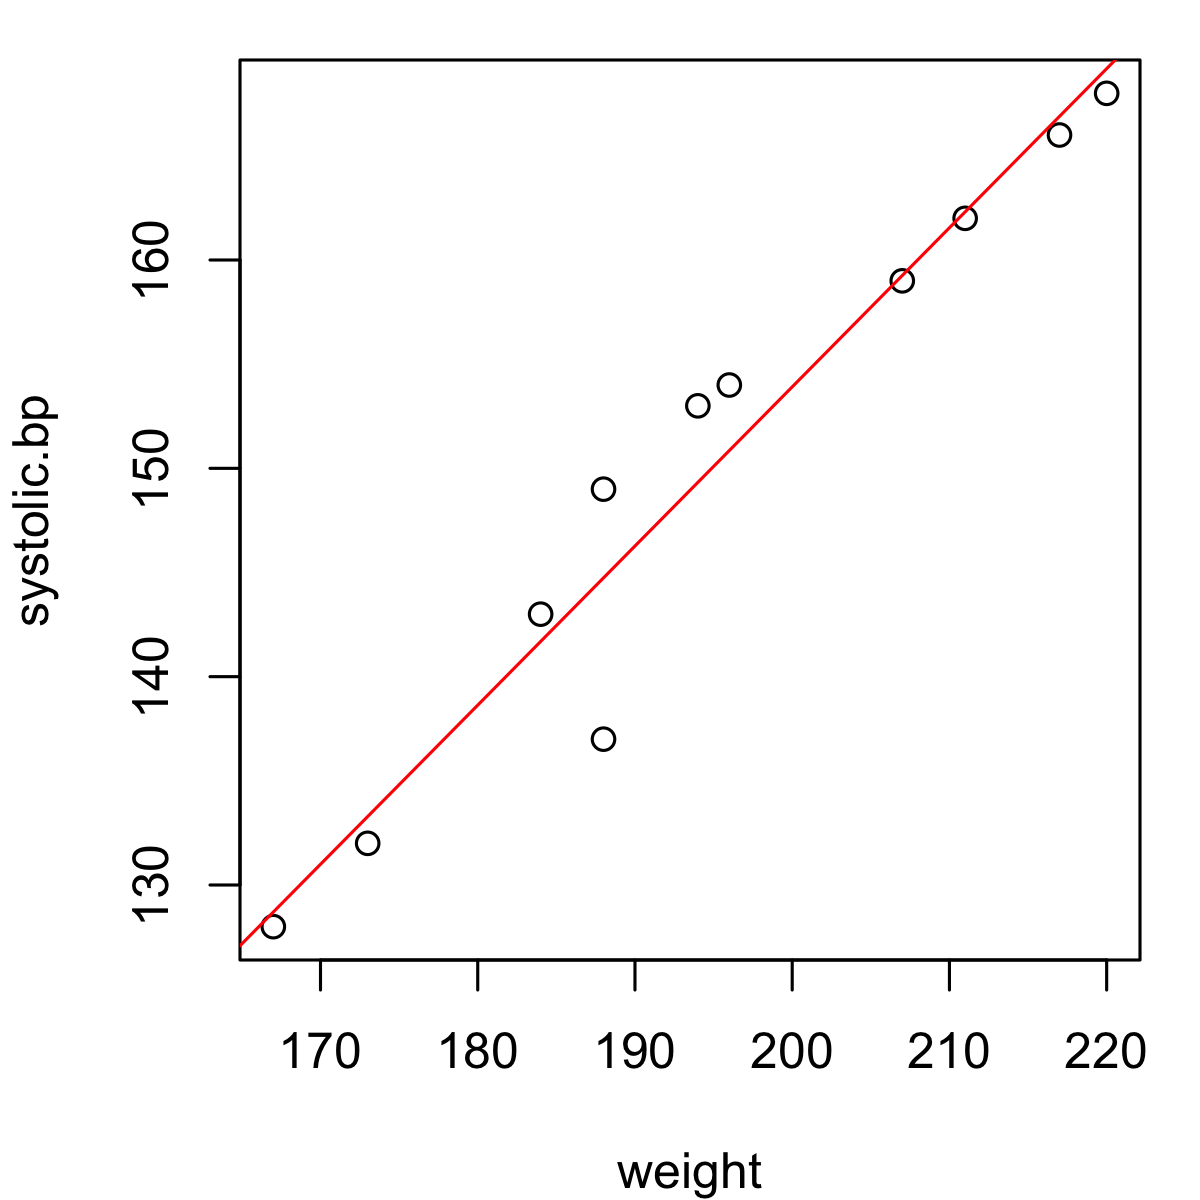
\includegraphics[width=0.38\textwidth]{img/systolic-bp-simple-plot-wmodel.png}\end{center}

\subsection{Coefficients and Standard Errors}

There are analytical expressions for the coefficients and standard errors of the coefficients in linear regression. They are:
\begin{align*} \hat{\beta} &= (X^T X)^{-1} X^T y \\
\hat{\text{Var}}(\hat{\beta}) &= \hat{\sigma}^2 (X^T X)^{-1}
\end{align*}
where our estimate of $\sigma^2$, $\hat{\sigma}^2$, is
$$ \hat{\sigma}^2 = \frac{1}{n-p-1} \sum_{i=1}^n (y^{(i)} - \hat{\beta}^T x^{(i)})^2.$$ Here is some awful-looking code that does these analytical calculations for our model.

\begin{center}
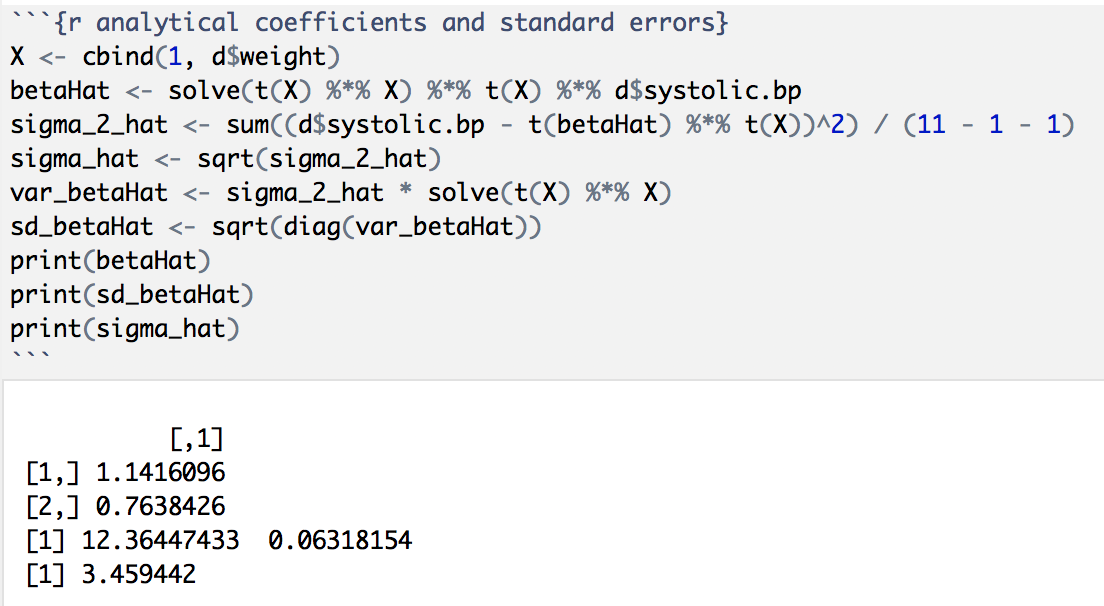
\includegraphics[width=0.8\textwidth]{img/analytical-coefficients-ses.png}
\end{center}

Do those numbers look familiar\footnote{If you want a more detailed explanation of where the coefficients and standard errors come from, see the explanation and code here: {\color{blue} https://stats.stackexchange.com/questions/44838/how-are-the-standard-errors-of-coefficients-calculated-in-a-regression}.}? :) 

\paragraph{Question 5} What does the model say will happen to a person's systolic blood pressure if his/her weight goes from 180 to 190 pounds? How about from 190 to 200 pounds? Is this realistic?

\vspace{50mm}

It turns out that we can perform a \textbf{hypothesis test} on each regression coefficient. Under the null hypothesis that the coefficient is zero and assuming $n$ is large enough, the quantity $\hat{\beta_j}/\text{se}(\hat{\beta}_j)$ will be distributed according to a Student's T distribution (see SC \#4 notes, Section 4.2.3) with $n-p$ degrees of freedom.

\begin{center}
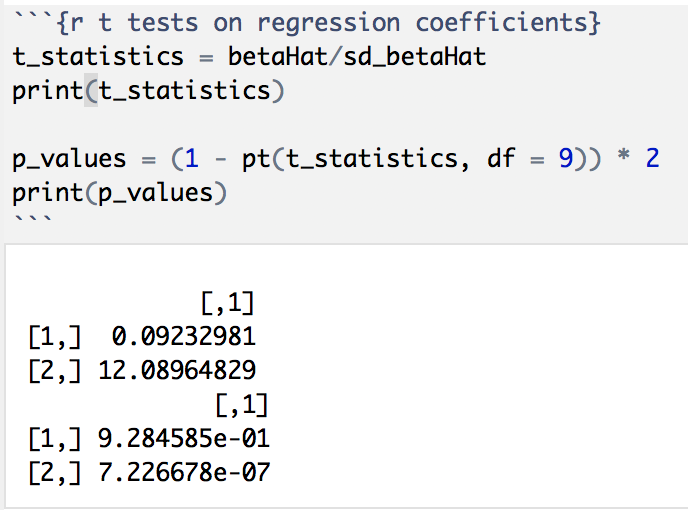
\includegraphics[width=0.5\textwidth]{img/t-tests-coefficients.png}
\end{center}

\subsection{Other Model Output}

The model also provides some other output. The quantity \textbf{R-squared} is defined as:
\begin{align*} R^2 &= 1 - \frac{\sum_{i=1}^n (y^{(i)} - \hat{y}^{(i)})^2}{\sum_{i=1}^n (y^{(i)} - \overline{y})^2} \\[3mm]
&=  1 - \frac{\sum_{i=1}^n (y^{(i)} - \hat{\beta}^T x^{(i)})^2}{\sum_{i=1}^n (y^{(i)} - \overline{y})^2} \end{align*}
or rather, the proportion of total variance in $y$ explained by the model. The \textbf{adjusted R-squared} is almost exactly the same except it fixes a source of bias in $R^2$, namely that $R^2$ will favor models with more parameters. Adjusted $R^2$ penalizes models with more parameters
\begin{align*}
 R^2_{\text{adj}} &= 1 - \frac{n-1}{n-p-1} \frac{\sum_{i=1}^n (y^{(i)} - \hat{y}^{(i)})^2}{\sum_{i=1}^n (y^{(i)} - \overline{y})^2} \\[3mm]
 &= 1 - (1 - R^2) \frac{n-1}{n-p-1}
\end{align*}
The \textbf{F-statistic} is the ratio of two variances: the variance explained by the model parameters (``sum of squares of regression'', or SSR) and the residual, or unexplained variance (``sum of squares of error'', or SSE). This ratio follows an $F$ distribution with $p$ and $n-p-1$ degrees of freedom. See R's \textbf{anova} function for more details. F-tests can be used to compare any two nested linear regression models. 
\newpage

%%%%%%%%%%%%%%%%%%%%%%%%%%%%%%%%%%%%%%%%%%%%%%%%%%%%%%%%%%%%%%%%%%%%%%%%%%%%%%%%

\section{Linearity: Anscombe's Quartet}

\textbf{Anscombe's Quartet} is a famous example of cases where linear regression models are applied in situations that do not fit the model assumptions, or where the conclusions of the model are unlikely to extrapolate to new datasets. The regression lines produced by fitting a linear regression model to each dataset are \emph{identical}.  

\begin{center}
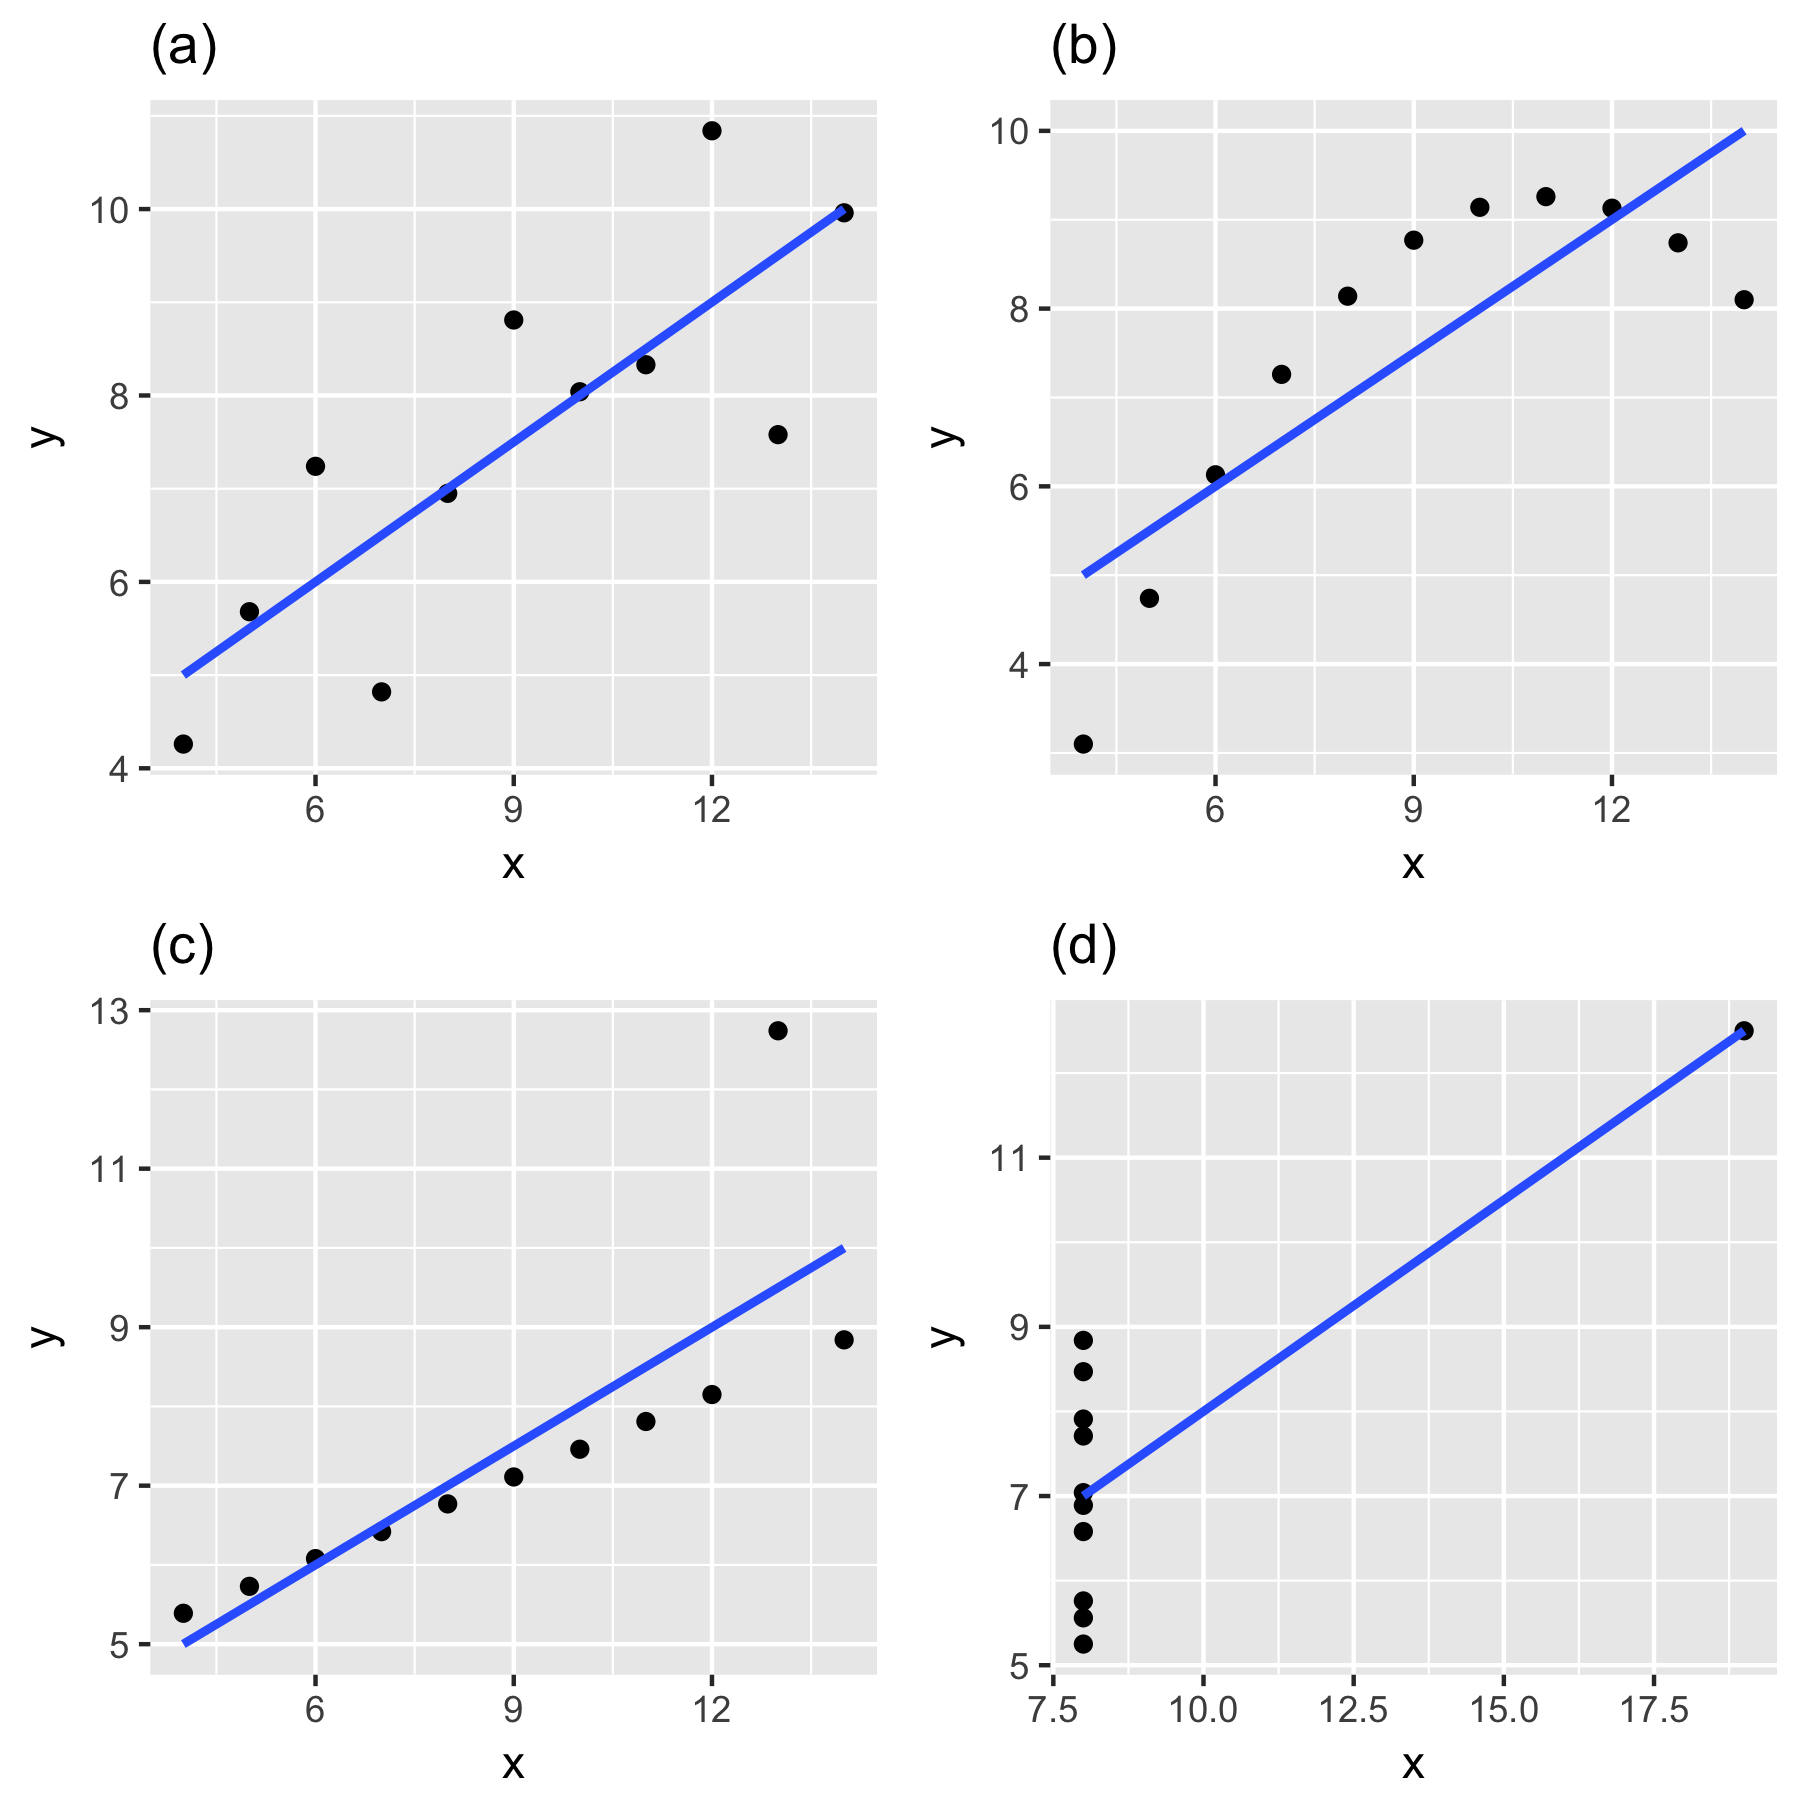
\includegraphics[width=0.8\textwidth]{img/anscombe.png}
\end{center}

\textbf{The most important thing you can do when building regression (or any) models is look at your data.}


\newpage

\paragraph{Question 6} What is a \textbf{residual} in a linear regression model? Using this definition, interpret the following diagnostic plots.

\begin{center}
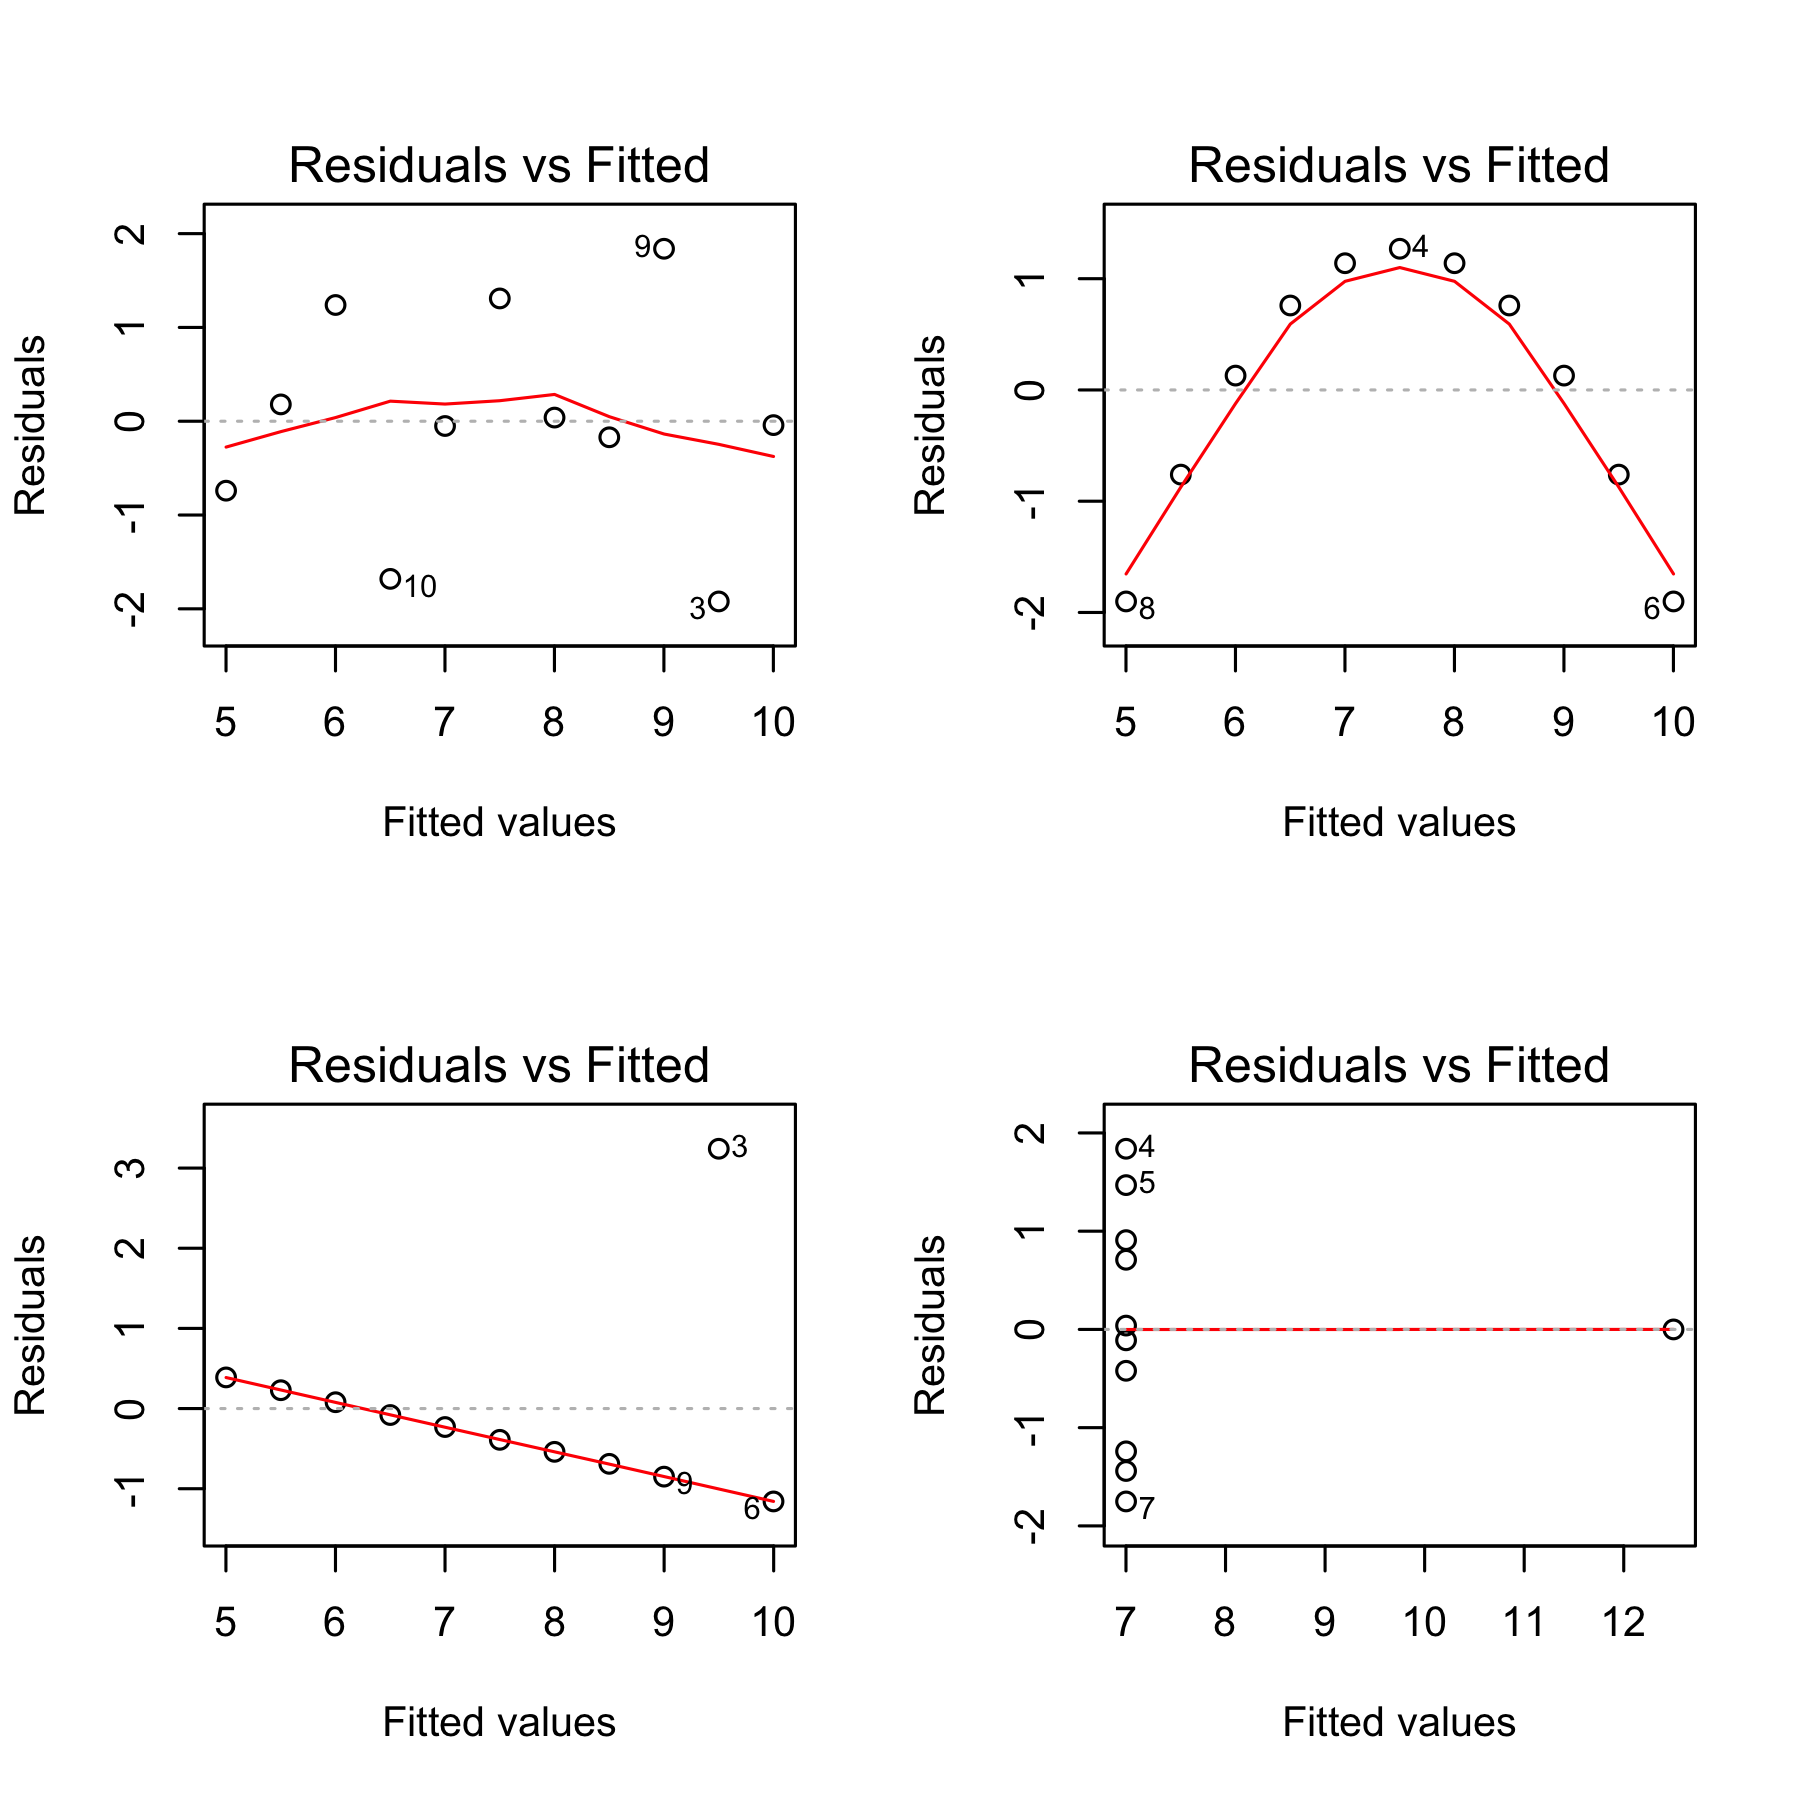
\includegraphics[width=0.9\textwidth]{img/anscombe-diagnostics-1.png}
\end{center}

\newpage

%%%%%%%%%%%%%%%%%%%%%%%%%%%%%%%%%%%%%%%%%%%%%%%%%%%%%%%%%%%%%%%%%%%%%%%%%%%%%%%%

\section{Transformations}

Violations of the linearity assumption in regression models typically lead to the most severe errors/lack of reproducibility. One way of combating this is to transform one or more of the predictors ($x$), the outcome ($y$), or both. Transformations sometimes also help with heteroskedasticity and non-normality of errors in linear regression models.

For example, gene expression data are often transformed using a log transformation to yield a distribution that looks more ``normal''.

\begin{center}
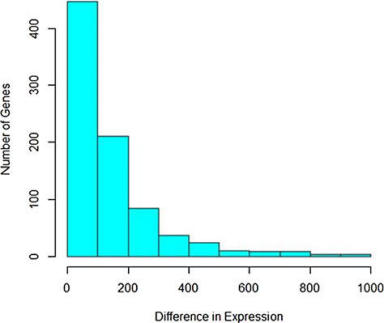
\includegraphics[width=0.32\textwidth]{img/gene-expression-histogram.jpg}
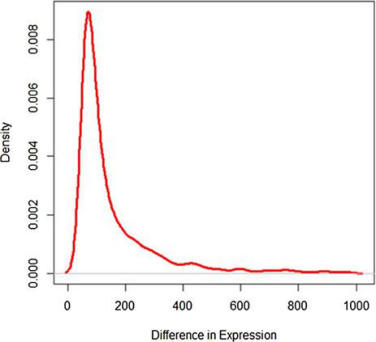
\includegraphics[width=0.32\textwidth]{img/gene-expression-density.jpg}
\end{center}
{\small Source: Anjum A, Jaggi S, Varghese E, Lall S, Bhowmik A, Rai A. (2016). Identification of Differentially Expressed Genes in RNA-seq Data of Arabidopsis thaliana: A Compound Distribution Approach. Journal of Computational Biology. 23.}

\begin{center}
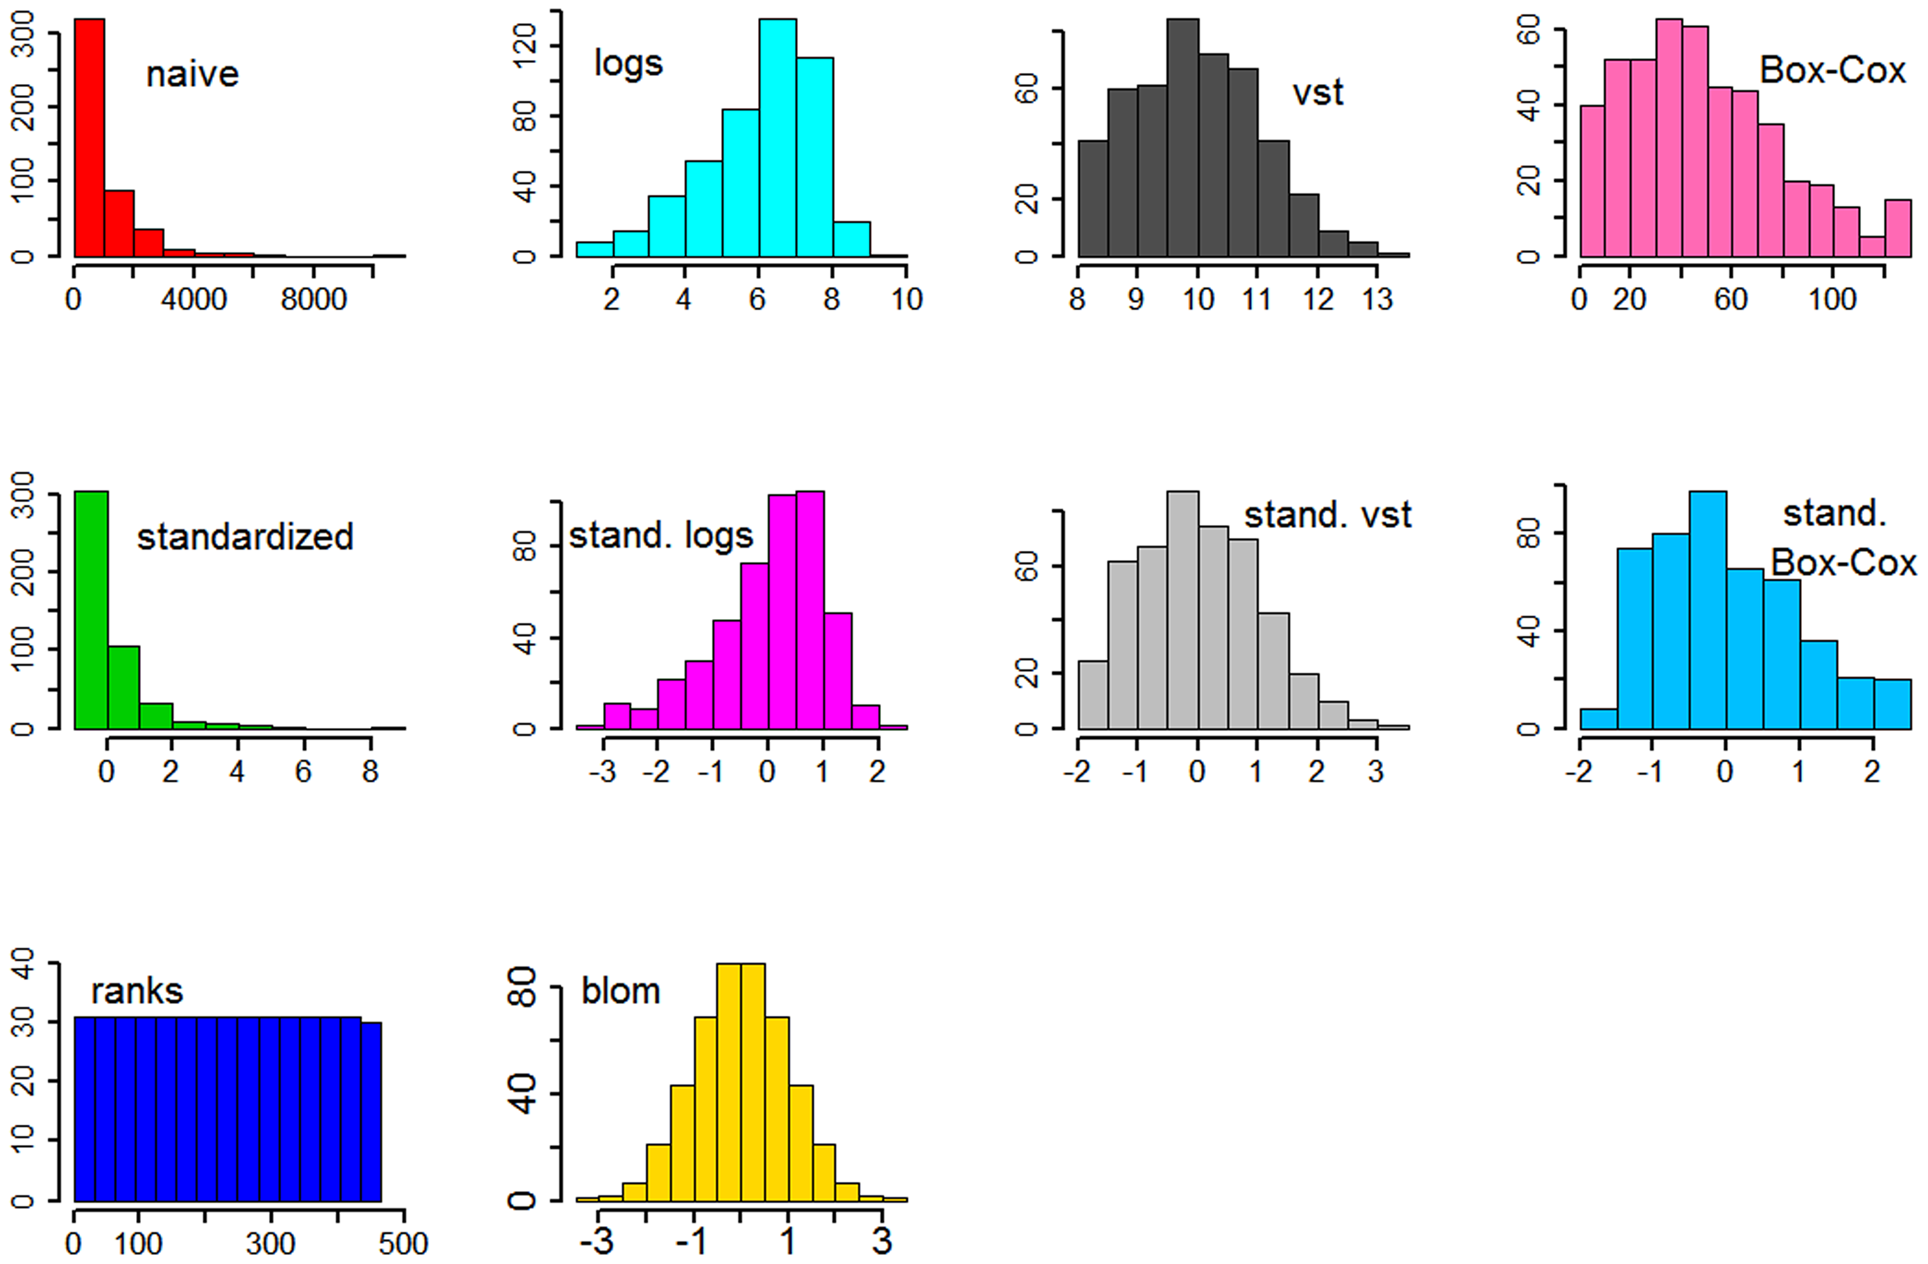
\includegraphics[width=0.7\textwidth]{img/gene-expression-transforms.png}
\end{center}
{\small Zwiener I, Frisch B, Binder H (2014) Transforming RNA-Seq Data to Improve the Performance of Prognostic Gene Signatures. PLoS ONE 9(1): e85150.}

It's useful to think of generalized linear models as a technique for transforming outcome variables in a principled way (see Appendix on GLMs).

Other possibilities for combating nonlinearity: 
\begin{itemize}
\item Add another covariate that is a nonlinear function of your existing covariate. Note: You can fit arbitrarily complex polynomials using this method, but they will generally extrapolate poorly to areas beyond the range of the sample data. Make sure you're only adding in terms if they make sense.
\item Maybe there's some other independent variable you should be adding, or an interaction term.
\end{itemize}

\textbf{The best transformations are those that actually make sense and reflect a true/plausible relationship.} 

\paragraph{Question 7} Below is some code for simulating gene expression as a function of a single predictor, $x$. Here the true relationship is that $y$ is linearly related to $\log_{1.5}(x)$. We don't know the true relationship, obviously, but we try a model that uses a $\log_2$ transformation of $y$. 
\begin{center}
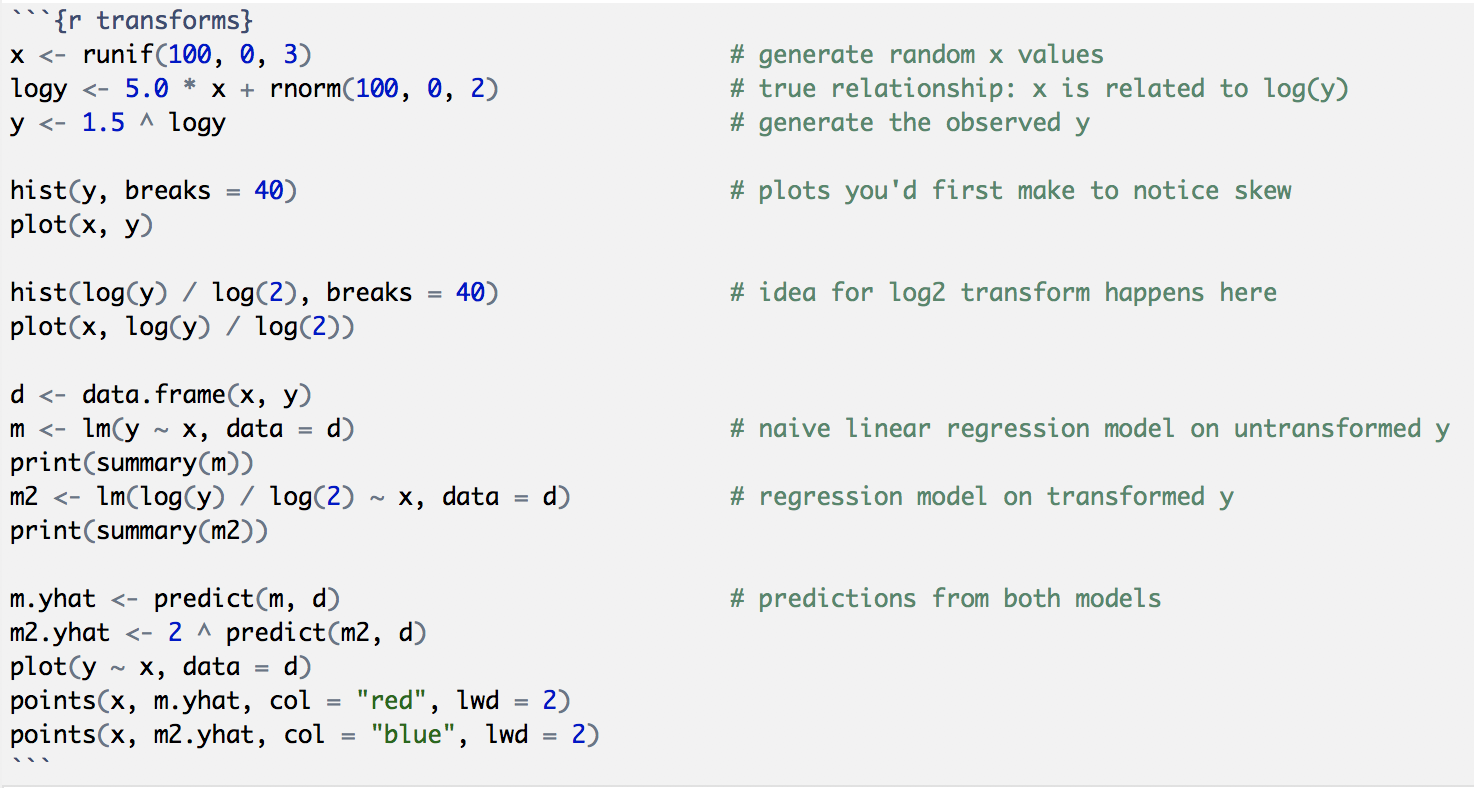
\includegraphics[width=\textwidth]{img/transform-sim-code.png}
\end{center}

\newpage

Here is the model output (naive model on top, log-transformed model on bottom):
\begin{center}
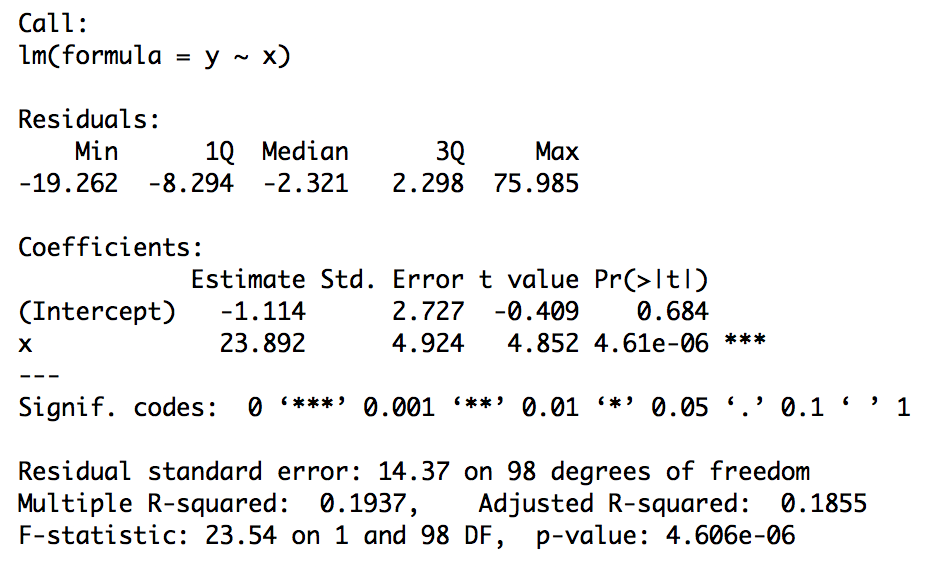
\includegraphics[width=0.7\textwidth]{img/transform-naive-model.png} \\[5mm]
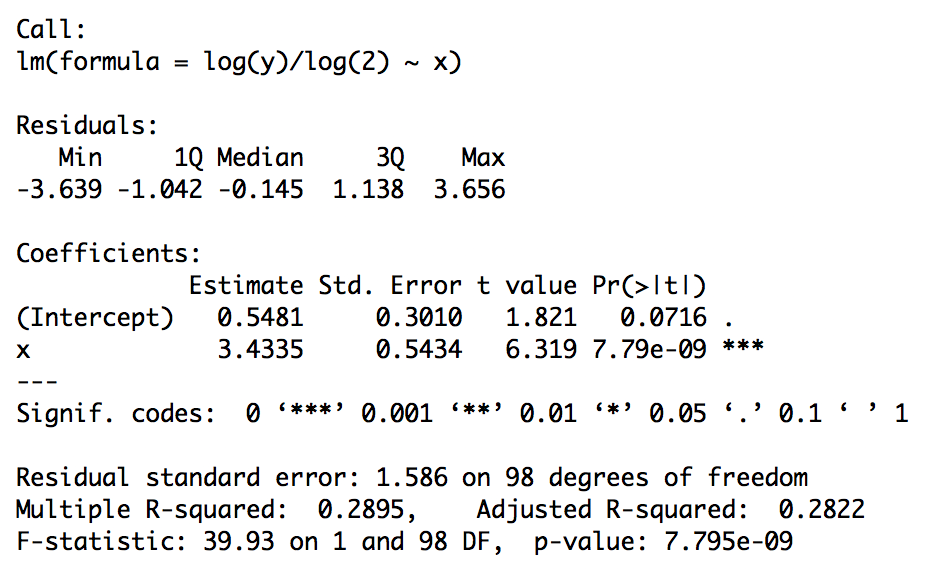
\includegraphics[width=0.7\textwidth]{img/transform-better-model.png}
\end{center}

You can see that both look sort of reasonable and both report a significant effect of $x$ on $y$. Had you not looked at the data, you would probably be happy with the naive model. But what do you think will happen when we try to use that model for prediction?

\begin{center}
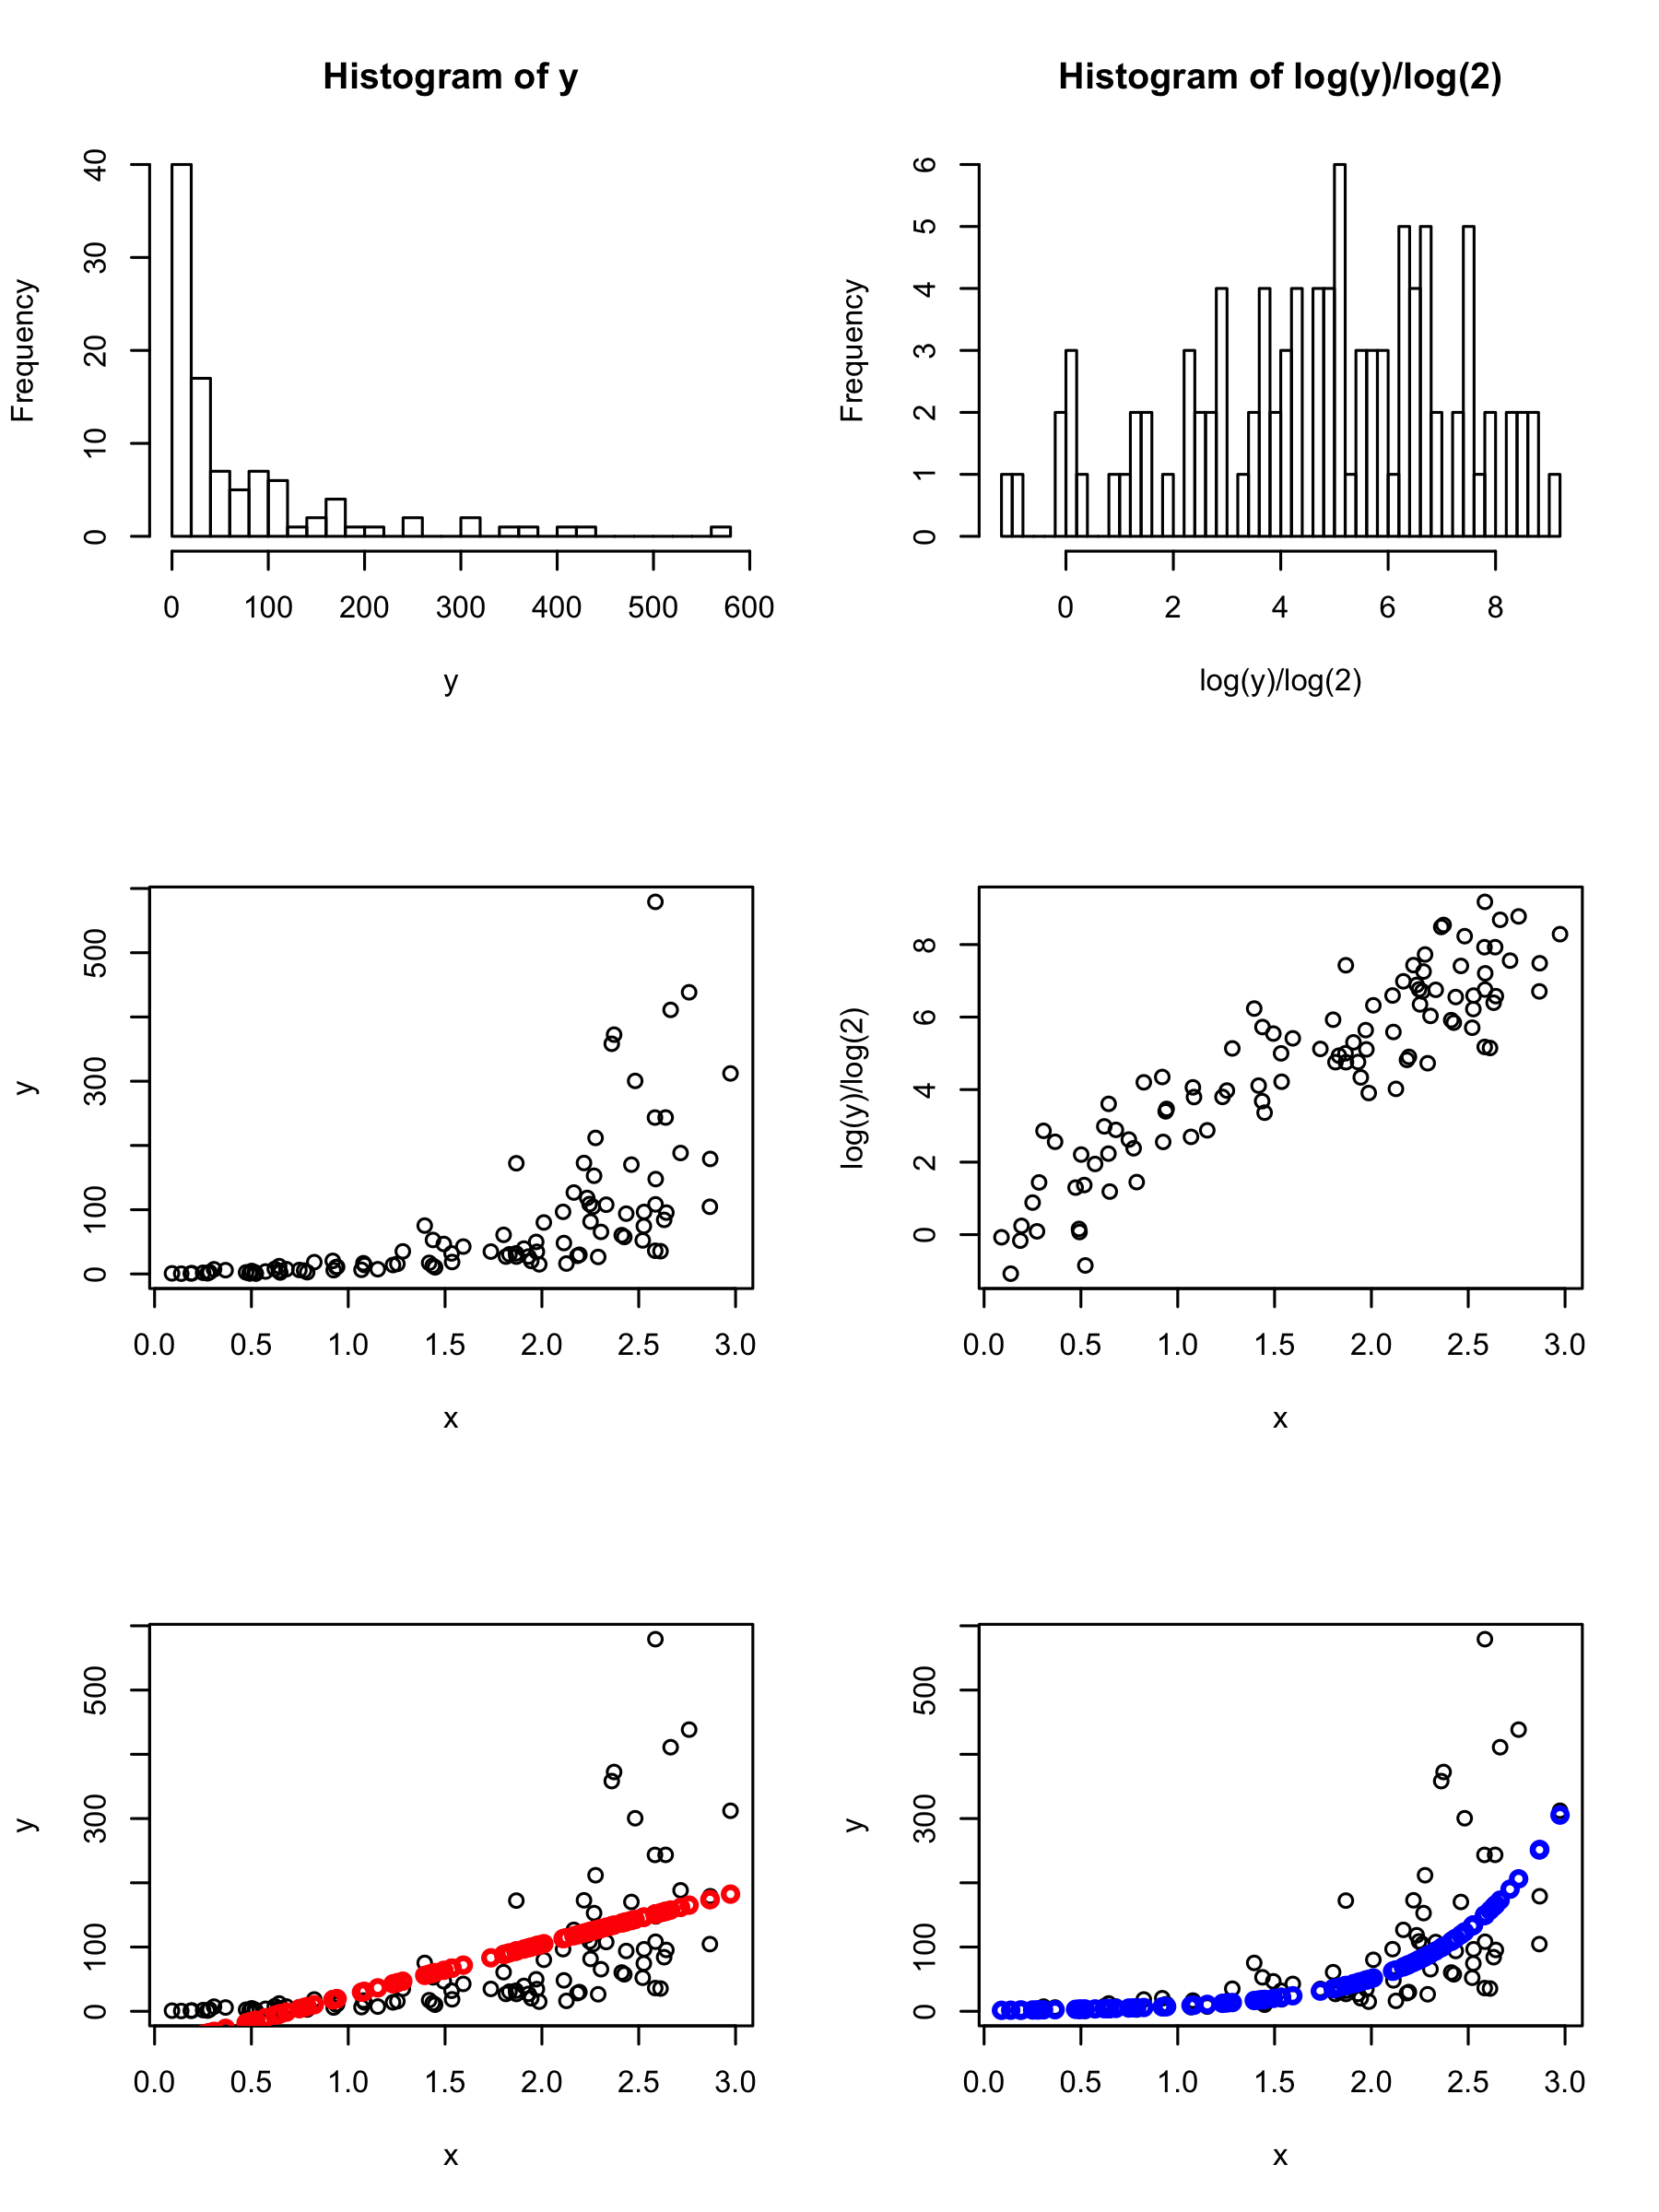
\includegraphics[width=0.85\textwidth]{img/transform-simulation-example.png}
\end{center}

\paragraph{What to Google:} Box-Cox transformations (and other power transformations); common transformations like log, square root, inverse; logistic and Poisson regression (and other GLMs)

%%%%%%%%%%%%%%%%%%%%%%%%%%%%%%%%%%%%%%%%%%%%%%%%%%%%%%%%%%%%%%%%%%%%%%%%%%%%%%%%

\section{Interpreting Logistic Regression Models}

A logistic regression model looks like this (also see Appendix):

$$ \log \frac{p}{1-p} = \beta_0 + \beta_1 x_1 + \dots + \beta_p x_p $$

where $p$ is the probability that our [binary] outcome is positive. You will note that there is no independent error term as there was in linear regression. That's because the variance and mean of a Bernoulli distribution are coupled, and depend only on $p$. 

Here's an example dataset for logistic regression. Data were collected on 189 women, 59 of which had low birth weight babies and 130 of which had normal birth weight babies.

\begin{center}
\texttt{
\begin{tabular}{ll}
\toprule
LOW & Low birth weight (0 = birth weight >= 2500 g; \\
     &                   1 = birth weight < 2500 g) \\
AGE & Age of mother in years \\
LWT & Mother's weight in pounds at last menstrual period \\
RACE & Race (1 = white, 2 = black, 3 = other) \\
SMOKE & Smoking status during pregnancy (1 = yes, 0 = no) \\
\bottomrule
\end{tabular}
}
\end{center}
{\small SOURCE: Hosmer and Lemeshow (2000) \emph{Applied Logistic Regression: Second Edition}. Data were collected at Baystate Medical Center, Springfield, Massachusetts during 1986.}

\paragraph{Question 8} Write down the form of a logistic regression model with LOW as the outcome and all the other covariates as predictors. What are $n$ and $p$ for this model/dataset?

\newpage

Here is the R summary for a logistic regression model fit on these data:

\begin{center}
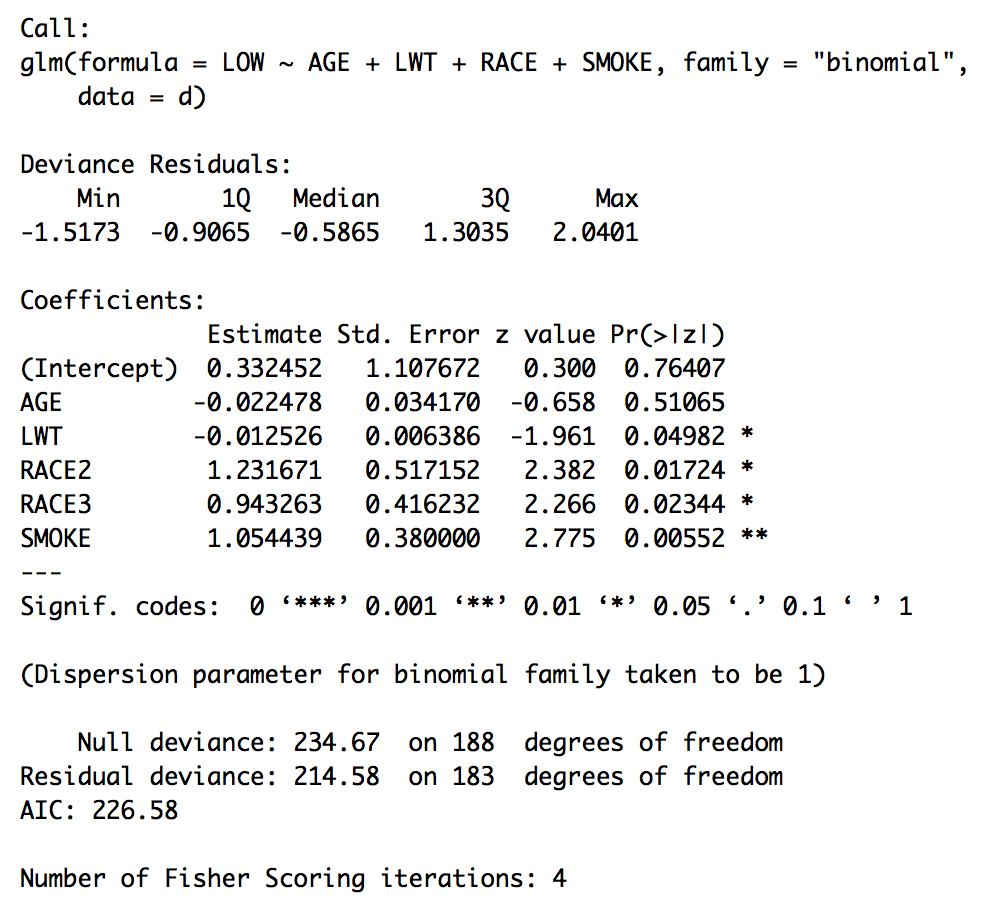
\includegraphics[width=0.7\textwidth]{img/low-bwt-model-1.png}
\end{center}

Generalized linear models like logistic regression estimate their coefficients using \textbf{maximum likelihood}, as opposed to least squares\footnote{Although linear regression is also a GLM and can be fit using maximum likelihood, which will yield the same estimates as for least squares; try using \texttt{glm} with \texttt{family = "normal"} in R.}. As such, their output looks quite different from that of linear regression, but a lot of the concepts are the same.

\paragraph{Question 9} What terms in the logistic regression output are analogous to the following?
\begin{itemize}
\item Coefficients and standard errors
\item T-tests for coefficients
\item Residuals
\item Residual standard error
\item Adjusted R-squared
\item F-statistic
\end{itemize}

\paragraph{Question 10} What is the probability that a 35-year-old, 160 pound, non-smoking black woman will have a low birthweight baby?

\vspace{50mm}

\paragraph{Question 11} What is the probability that a white woman her same age, weight, and smoking status will have a low birthweight baby?

\vspace{50mm}

\paragraph{Question 12} What is the odds ratio for having a low-birthweight baby between two women of the same age, weight, and race, one of which smokes and the other of which does not?

\vspace{40mm}

\paragraph{What to Google:} deviance; deviance residual; likelihood ratio test; Fisher scoring
\newpage

%%%%%%%%%%%%%%%%%%%%%%%%%%%%%%%%%%%%%%%%%%%%%%%%%%%%%%%%%%%%%%%%%%%%%%%%%%%%%%%%

\section{Correlations, Group Structure, Repeated Measures}

Often we encounter data where the independence assumption for the errors is violated. This can happen in several ways. The good news is that usually we are aware when this is happening because of the way data are collected.

\paragraph{Question 13} List three ways the independence assumption can be violated in real datasets.

% batch effects for experimental runs (e.g. microarrays)
% repeated measures on same patient
% seasonality/cohort effects

\vspace{30mm}

Here is an example of a synthetic dataset with hidden structure. If we just plot $x$ vs. $y$, it looks like there is nothing going on (left) but if we stratified on group identity (right), the data would clearly suggest five separate linear regression models.

\begin{center}
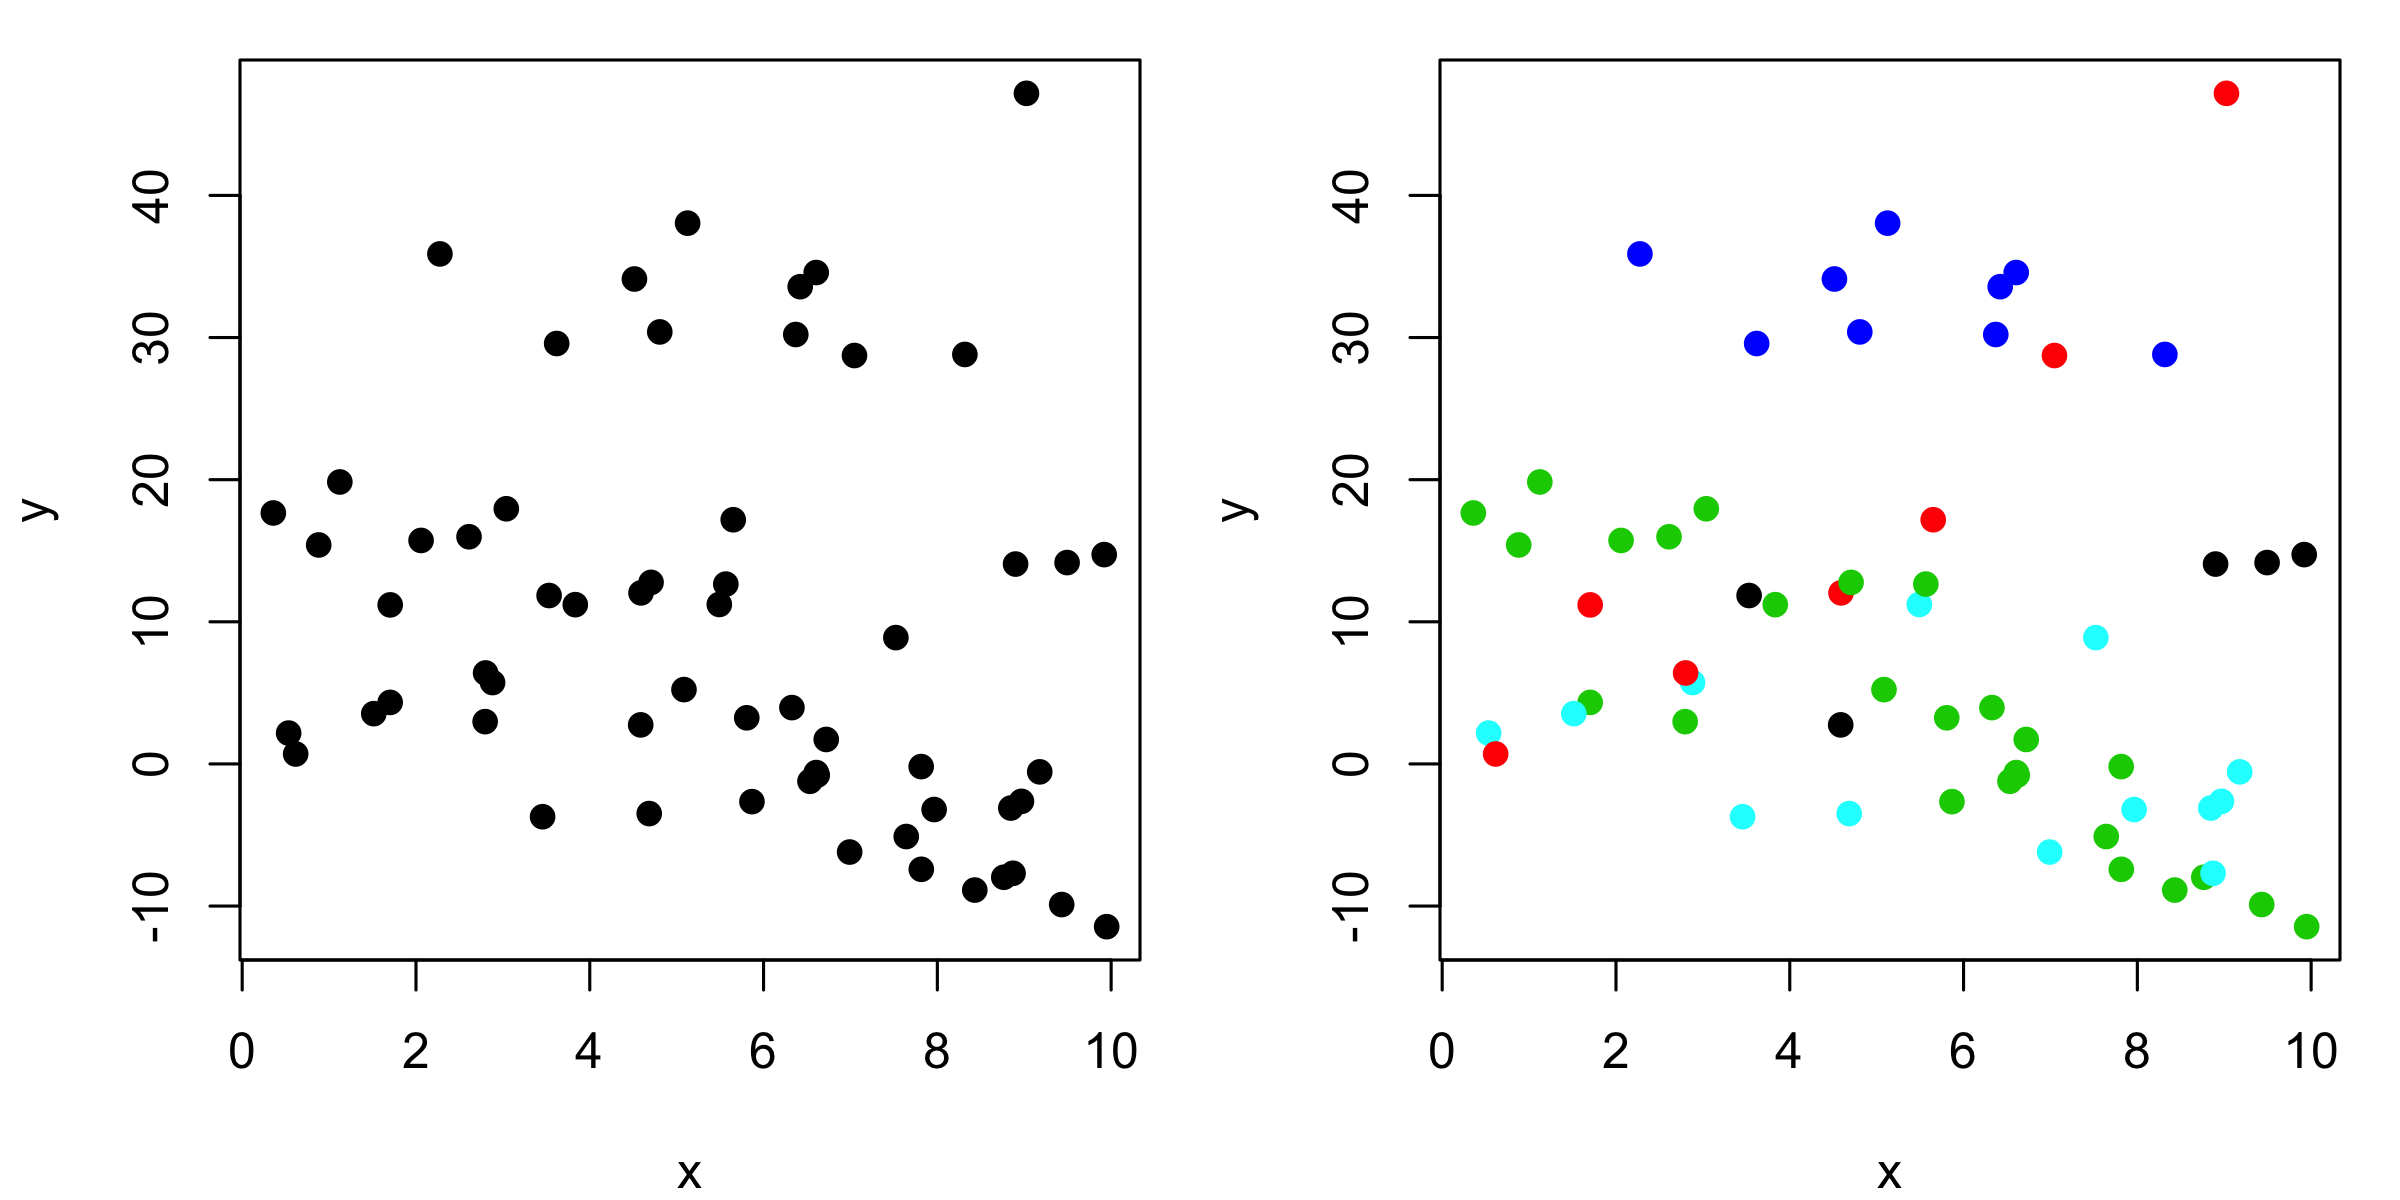
\includegraphics[width=0.85\textwidth]{img/correlated-plots.png}
\end{center}

\paragraph{Question 14} Write down (a) a naive linear regression model that just regresses $y$ on $x$ without considering group identity, (b) a model that has different intercepts for the different groups, (c) a model that has different slopes \emph{and} different intercepts for the different groups. What do you notice about the number of parameters in these three cases?

\newpage

Here is the code that generated these data:
\begin{center}
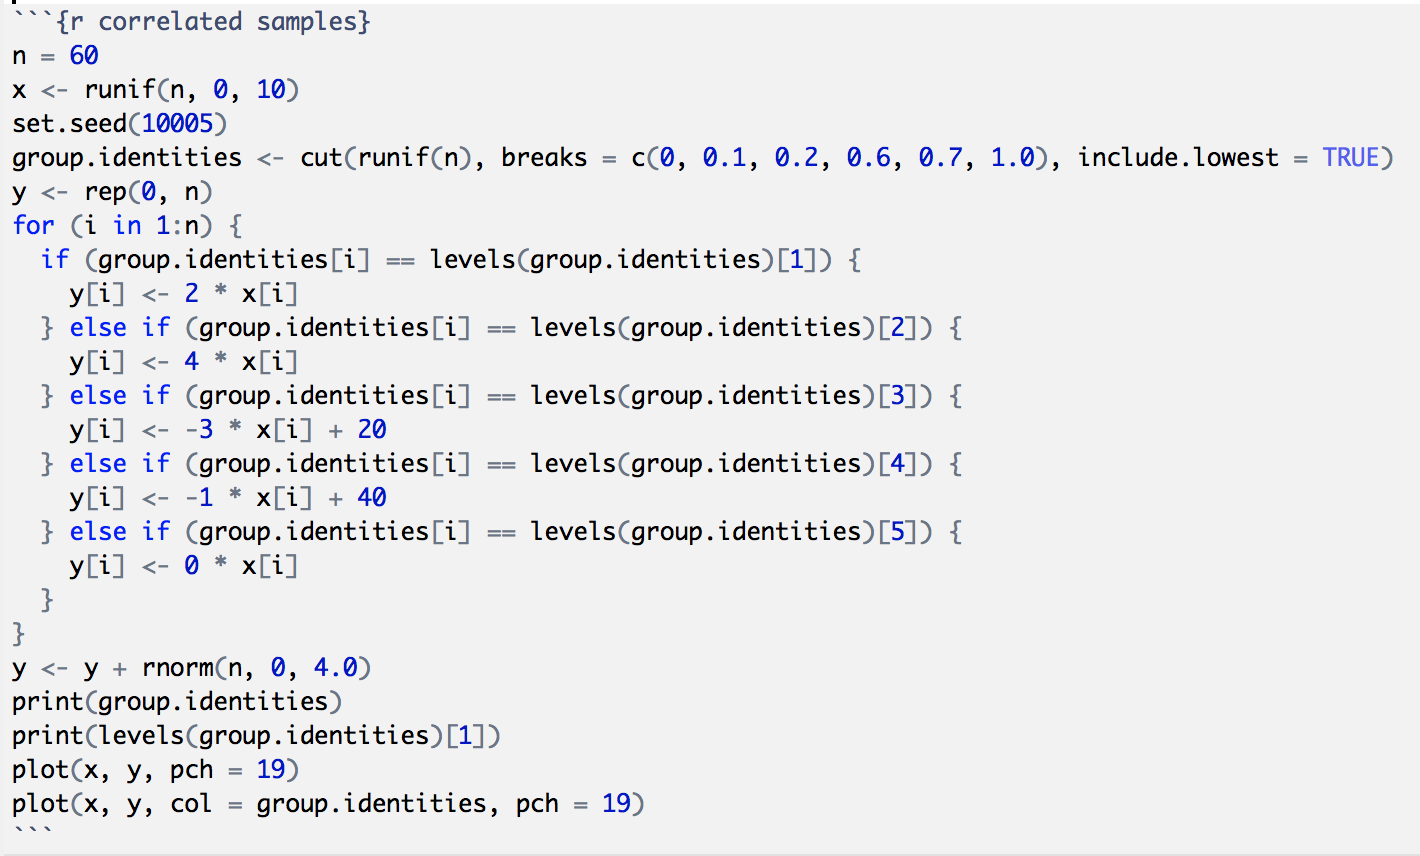
\includegraphics[width=0.9\textwidth]{img/code-hierarchical-model.png}
\end{center}

And here are the summary outputs from the three models we wrote down in Question 12, with the R calls that built the models shown first:

\begin{center}
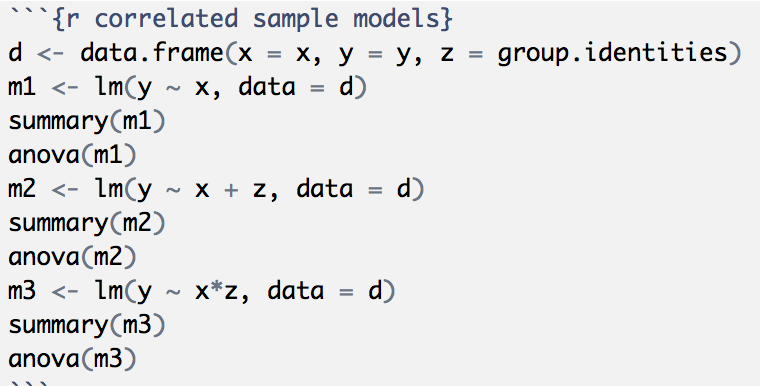
\includegraphics[width=0.6\textwidth]{img/code-models-123.png}
\end{center}

\begin{center}
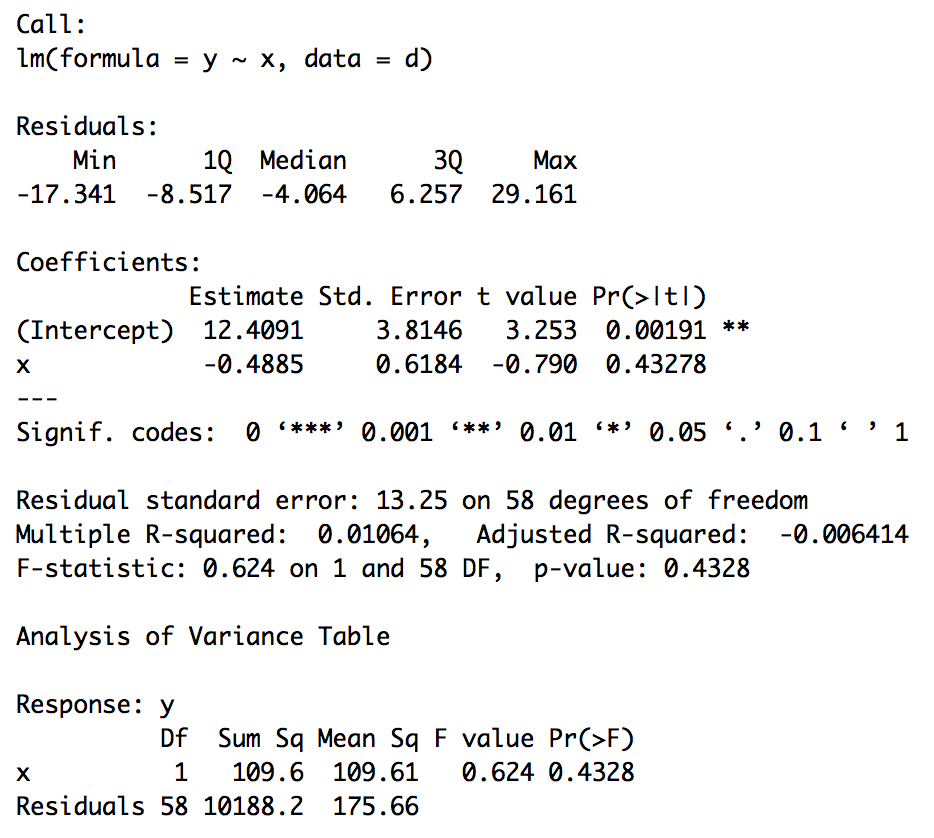
\includegraphics[width=0.6\textwidth]{img/model-1-output.png}
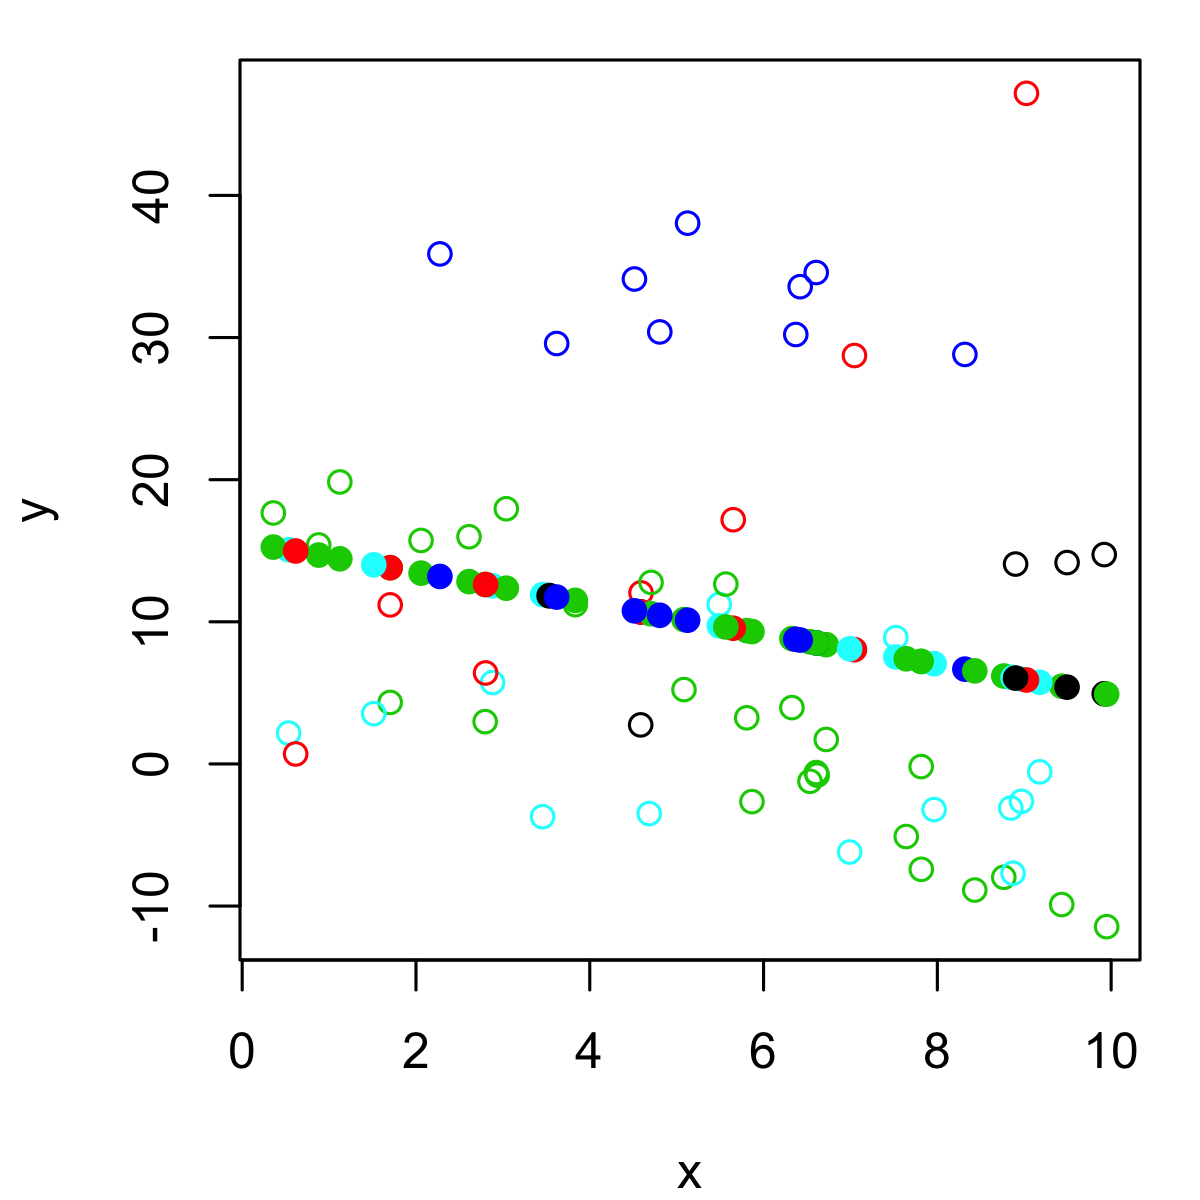
\includegraphics[width=0.37\textwidth]{img/model-1-predictions.png}
\end{center}

\begin{center}
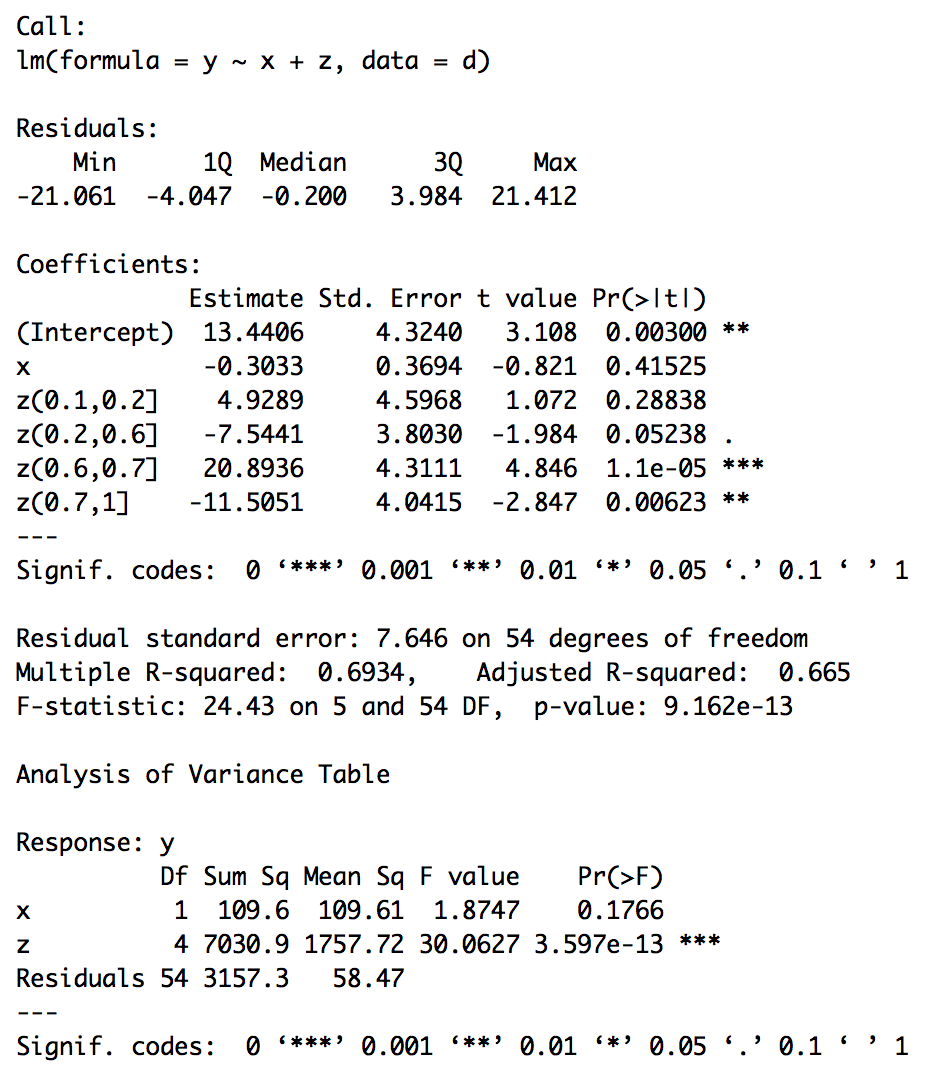
\includegraphics[width=0.6\textwidth]{img/model-2-output.png}
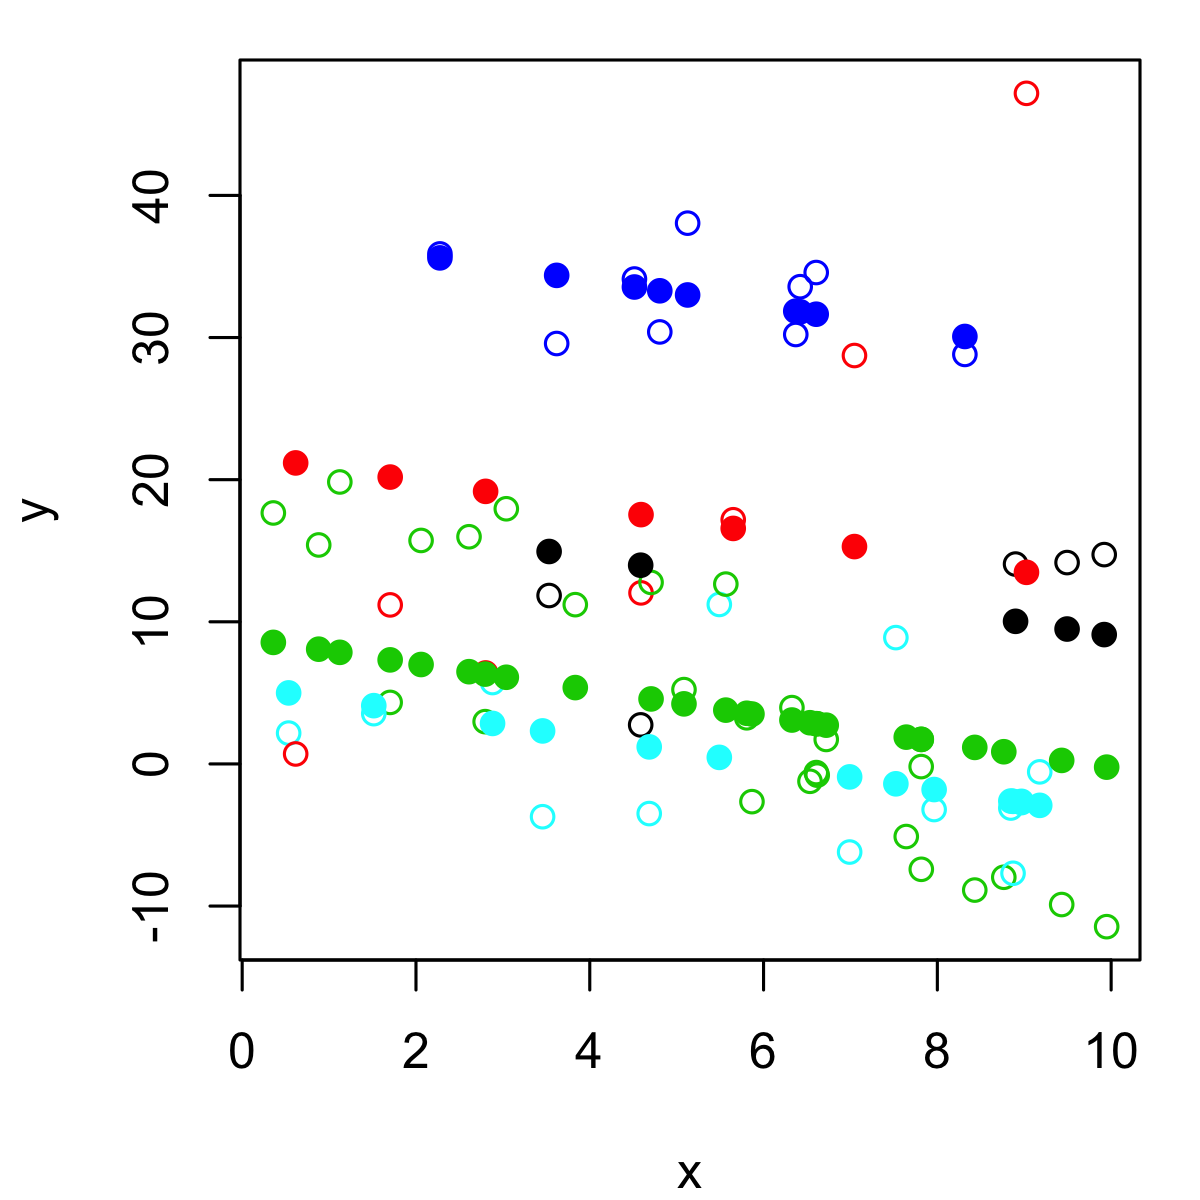
\includegraphics[width=0.37\textwidth]{img/model-2-predictions.png}
\end{center}

\begin{center}
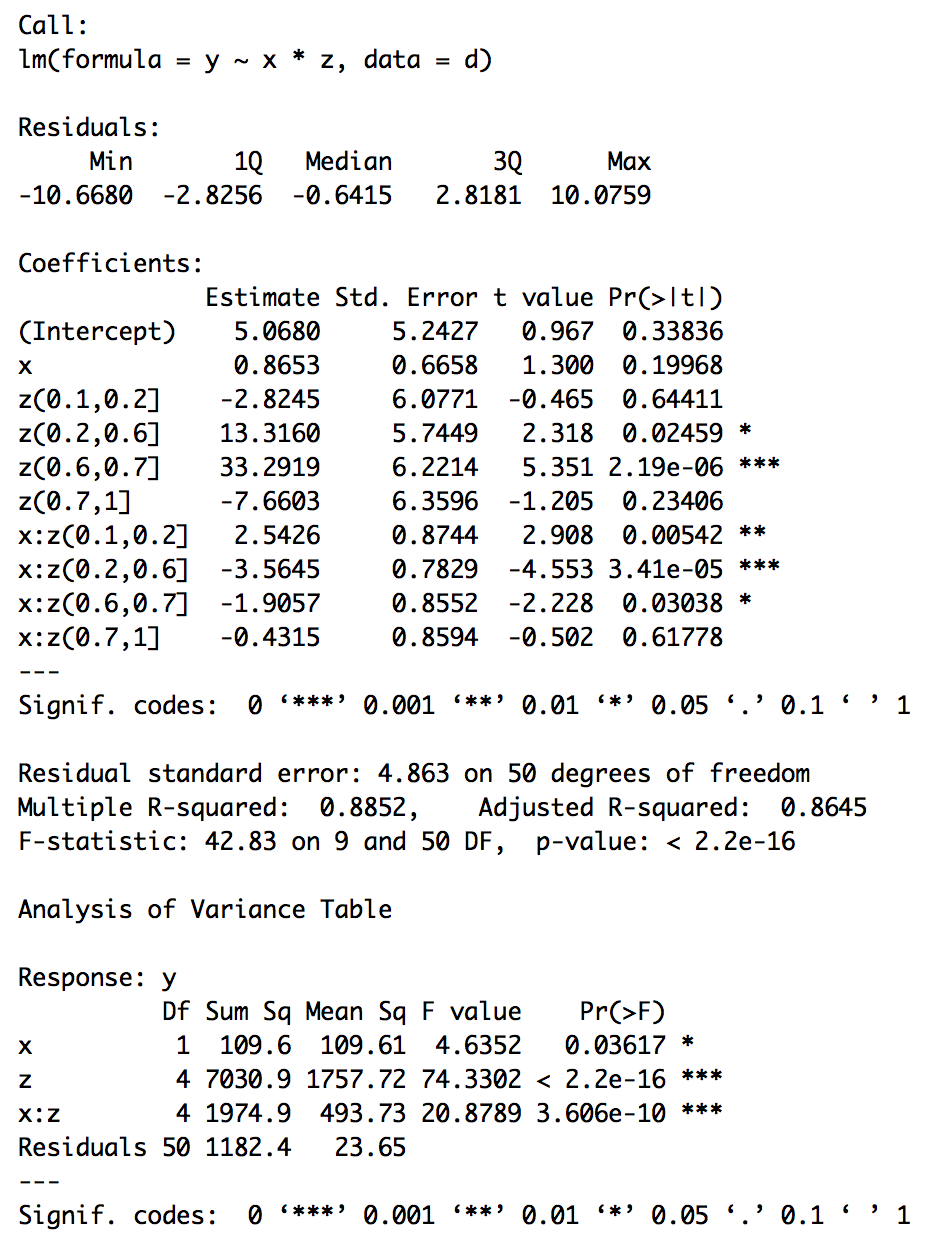
\includegraphics[width=0.6\textwidth]{img/model-3-output.png}
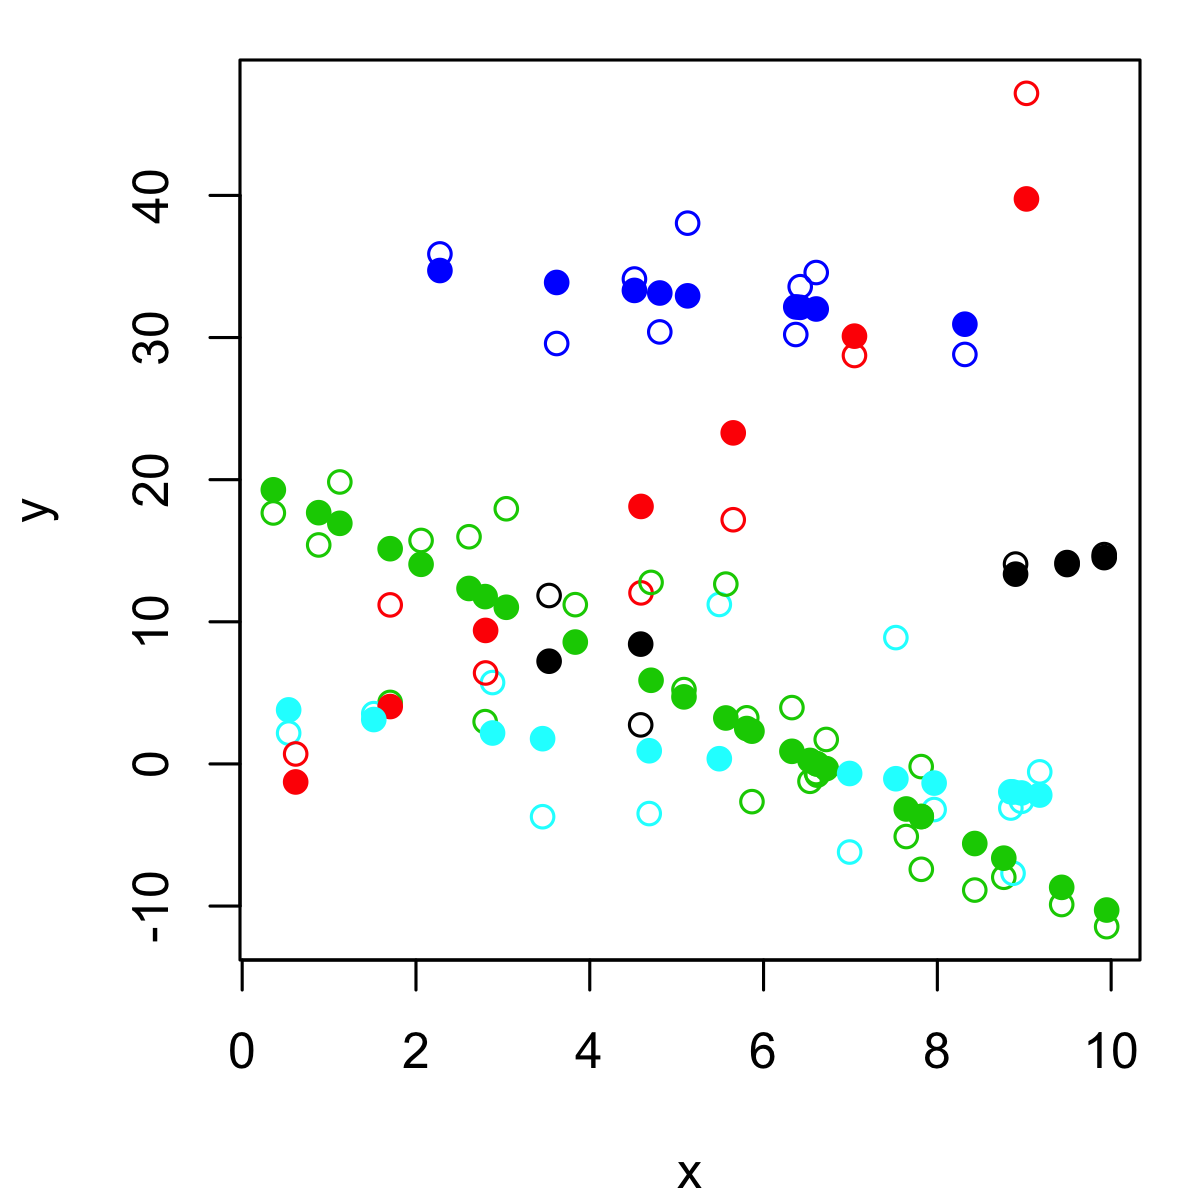
\includegraphics[width=0.37\textwidth]{img/model-3-predictions.png}
\end{center}

\paragraph{What to Google:} Linear mixed models; mixed effects models; random effects models; Generalized Estimating Equations (GEEs); hierarchical modeling; multi-level modeling; hierarchical Bayesian modeling; repeated measures. The field of \textbf{time-series analysis} is its own thing with its own theory and set of things to Google: ARIMA models; autoregressive models (same thing); stochastic processes; Bayesian time series models.

\newpage

%%%%%%%%%%%%%%%%%%%%%%%%%%%%%%%%%%%%%%%%%%%%%%%%%%%%%%%%%%%%%%%%%%%%%%%%%%%%%%%%

\section{Collinearity of Predictors}

Predictors are collinear when one is (or is close to being) a linear combination of one or more other predictors. In this case, the model coefficients may change erratically in response to small changes in the model or the data. Multicollinearity will generally not reduce the predictive power or reliability of the model as a whole; it only affects calculations regarding individual predictors. (See Wikipedia: ``Multicollinearity'')

Here is the same dataset of systolic blood pressure vs. weight that we looked at earlier, except now we have a new covariate: age.

\begin{center}
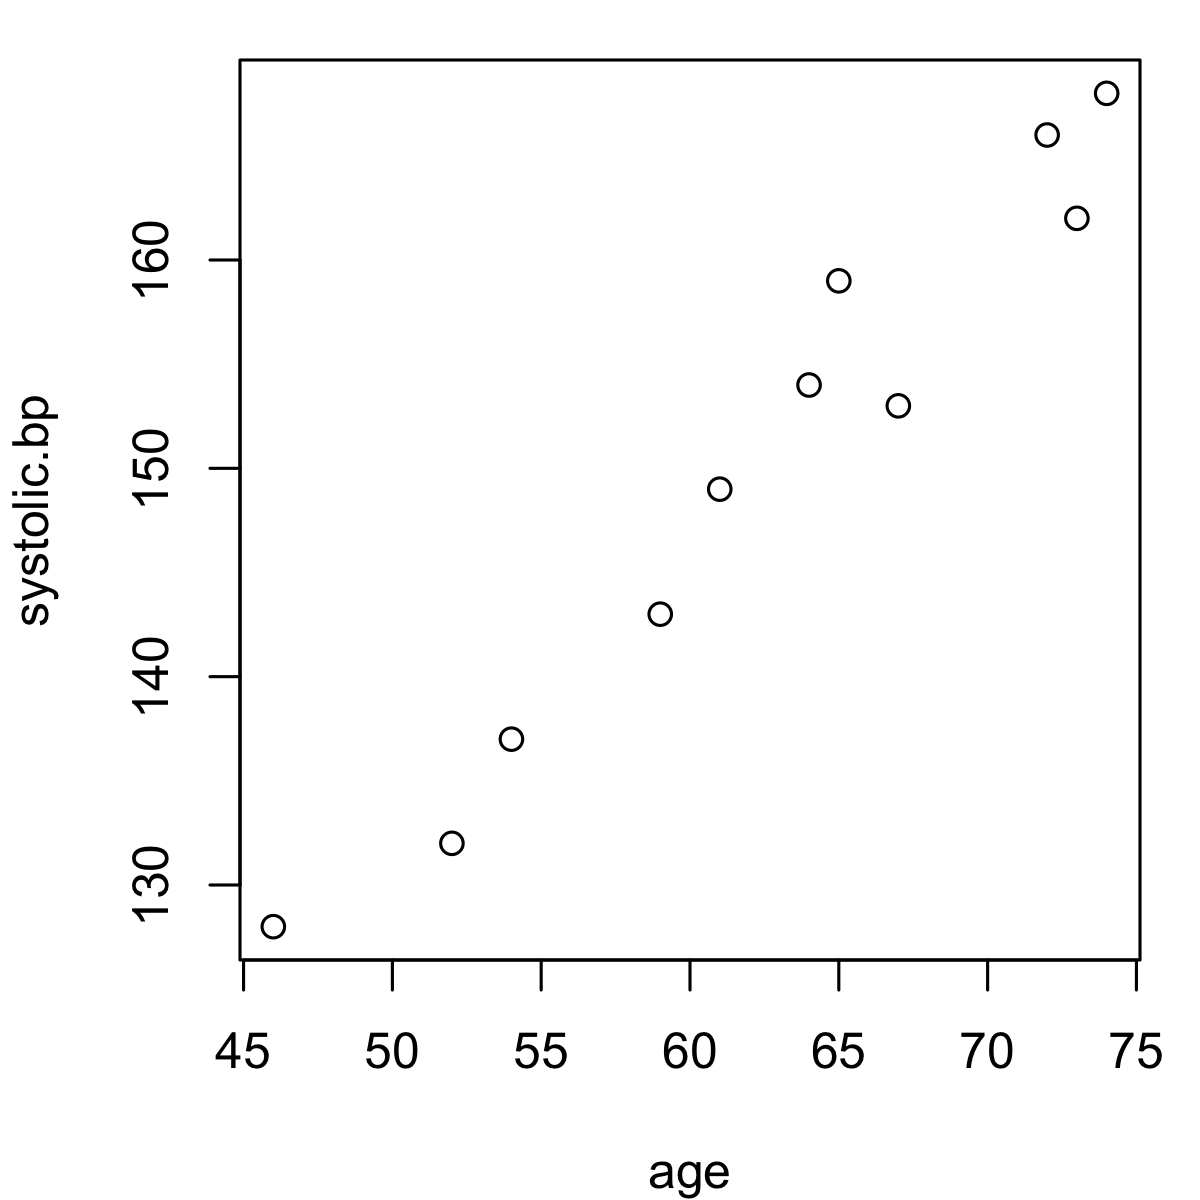
\includegraphics[width=0.32\textwidth]{img/sample-systolic-bp-1.png}
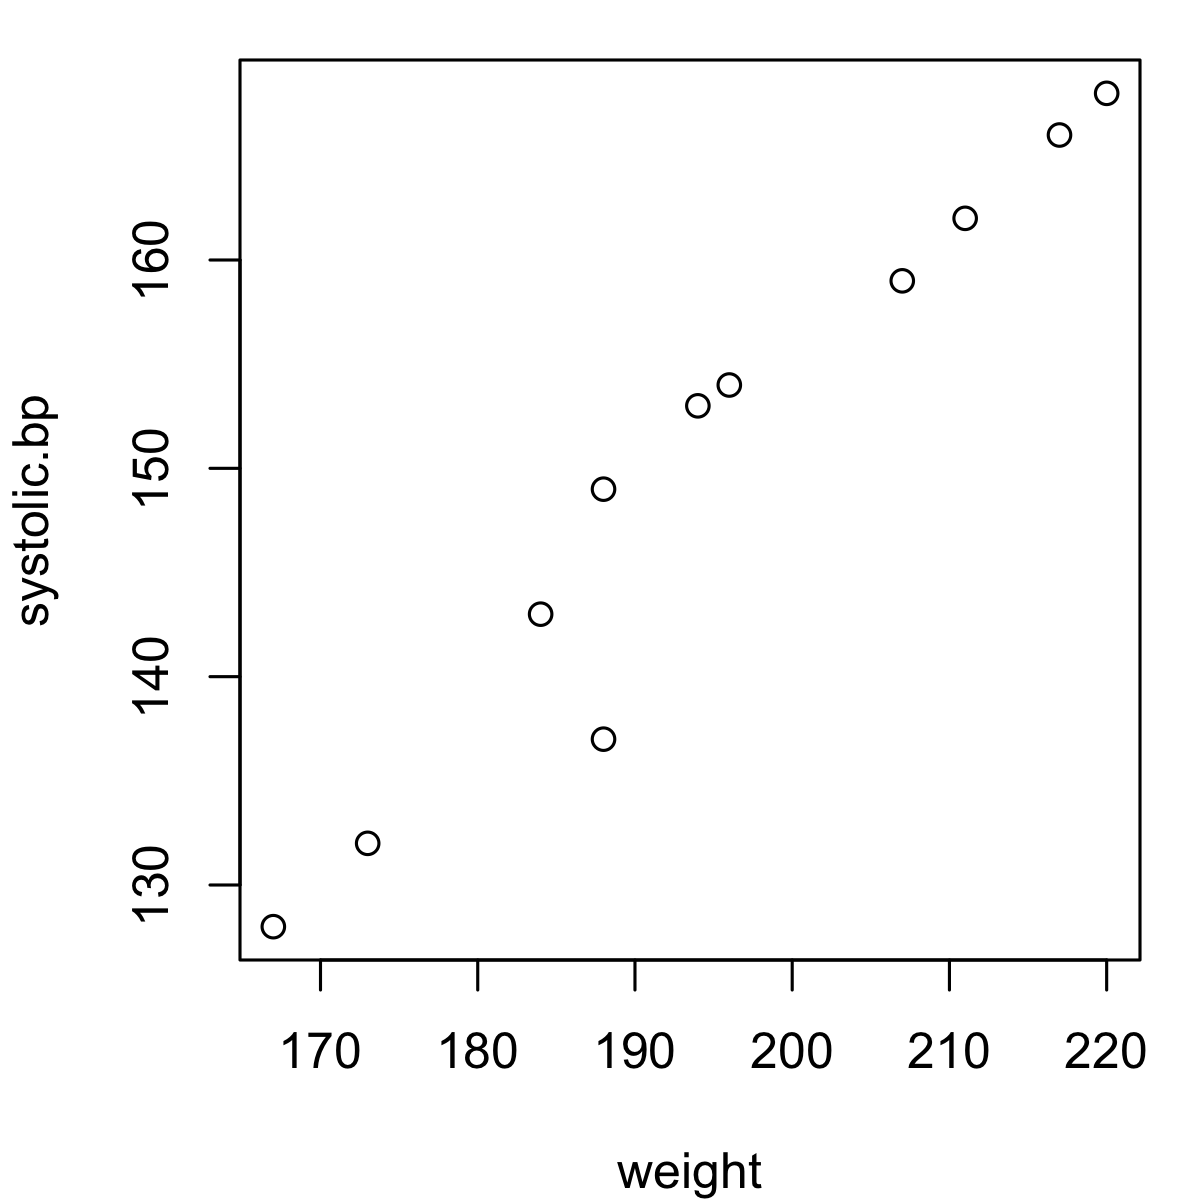
\includegraphics[width=0.32\textwidth]{img/systolic-bp-simple-plot.png}
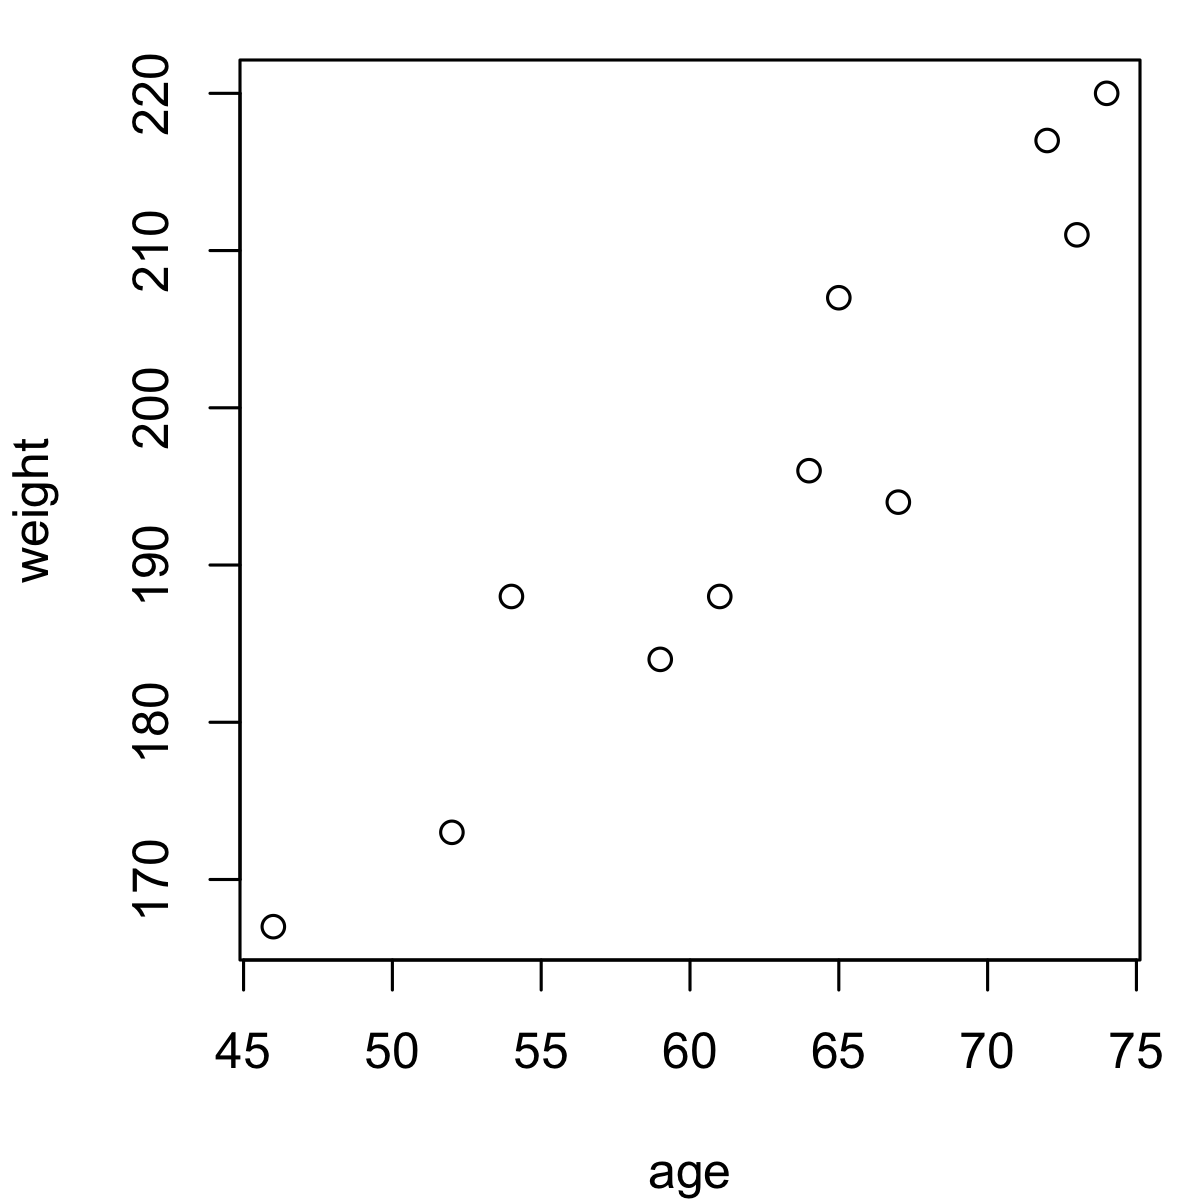
\includegraphics[width=0.32\textwidth]{img/sample-systolic-bp-3.png}
\end{center}

Here are two univariate models and one bivariate model, all fit to the same dataset:

\begin{center}
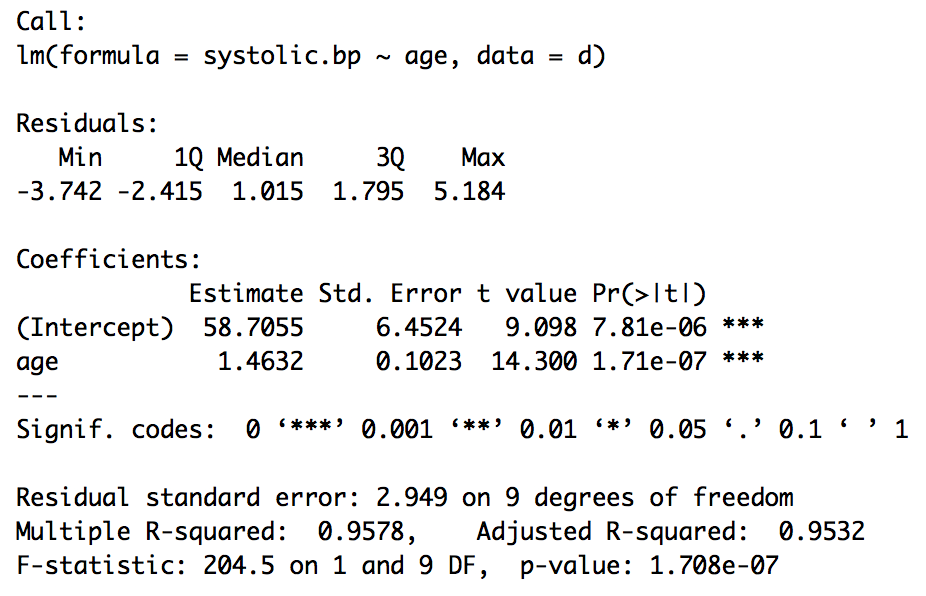
\includegraphics[width=0.7\textwidth]{img/collin-model-1.png}\\[5mm]
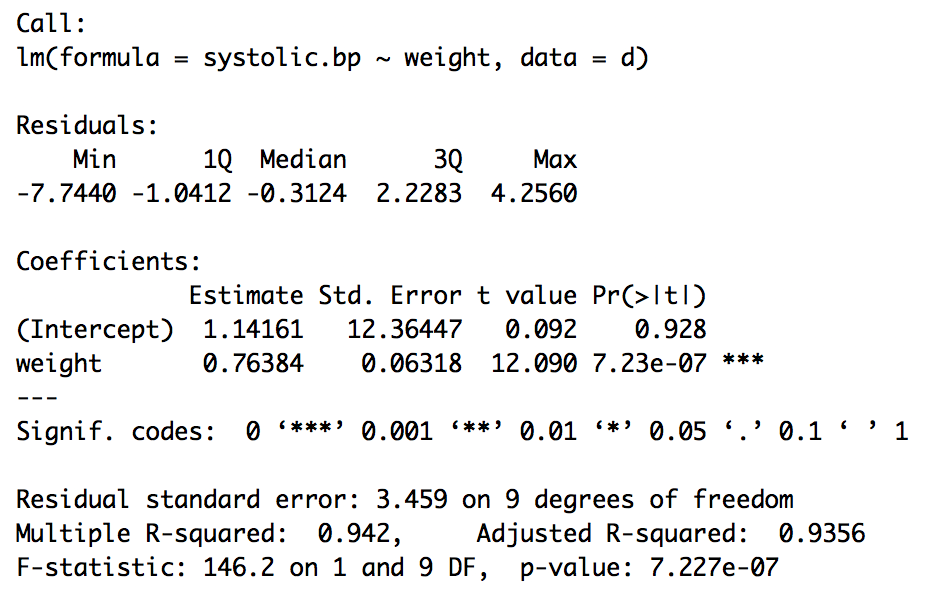
\includegraphics[width=0.7\textwidth]{img/collin-model-2.png}\\[5mm]
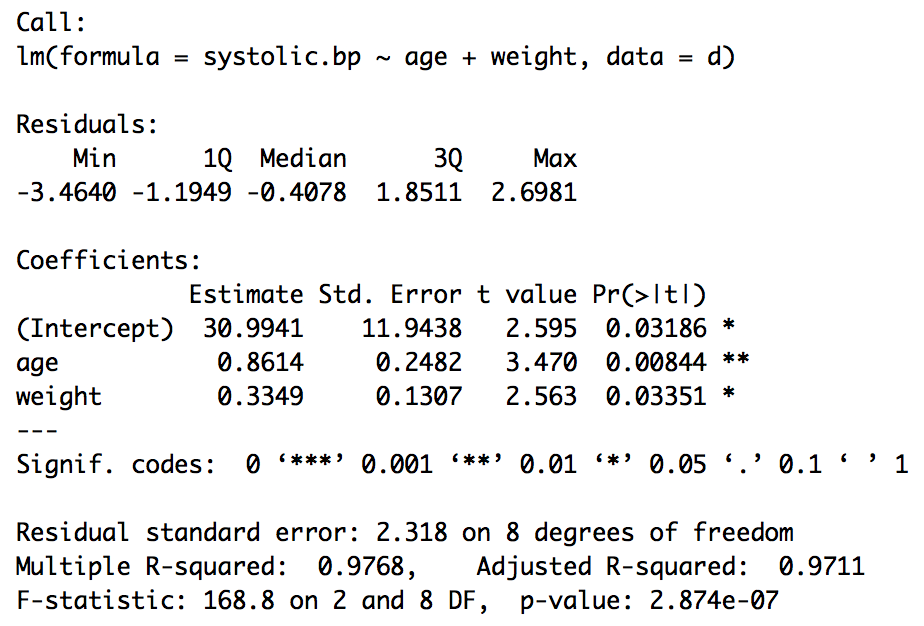
\includegraphics[width=0.7\textwidth]{img/collin-model-3.png}
\end{center}

\paragraph{Question 15} What do you notice about the standard errors of the coefficients? Why does this happen? (See formula for variance of coefficients in linear regression.)

\newpage

Here's what happens when we start randomly perturbing the dataset:

\begin{center}
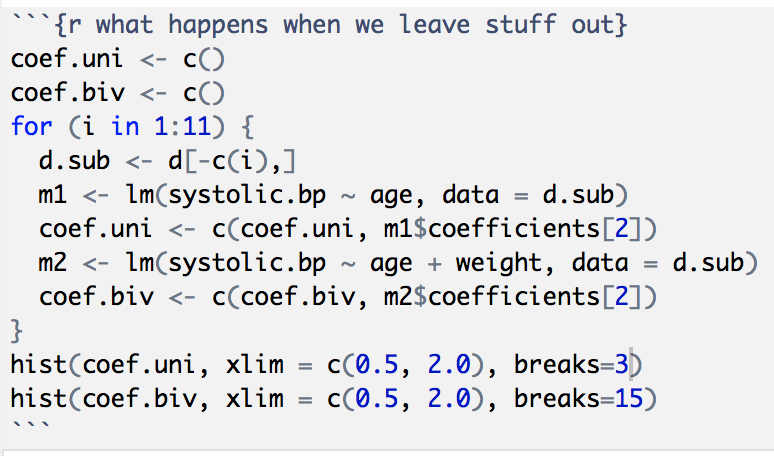
\includegraphics[width=0.6\textwidth]{img/coef-perturb-code.png}
\end{center}

\begin{center}
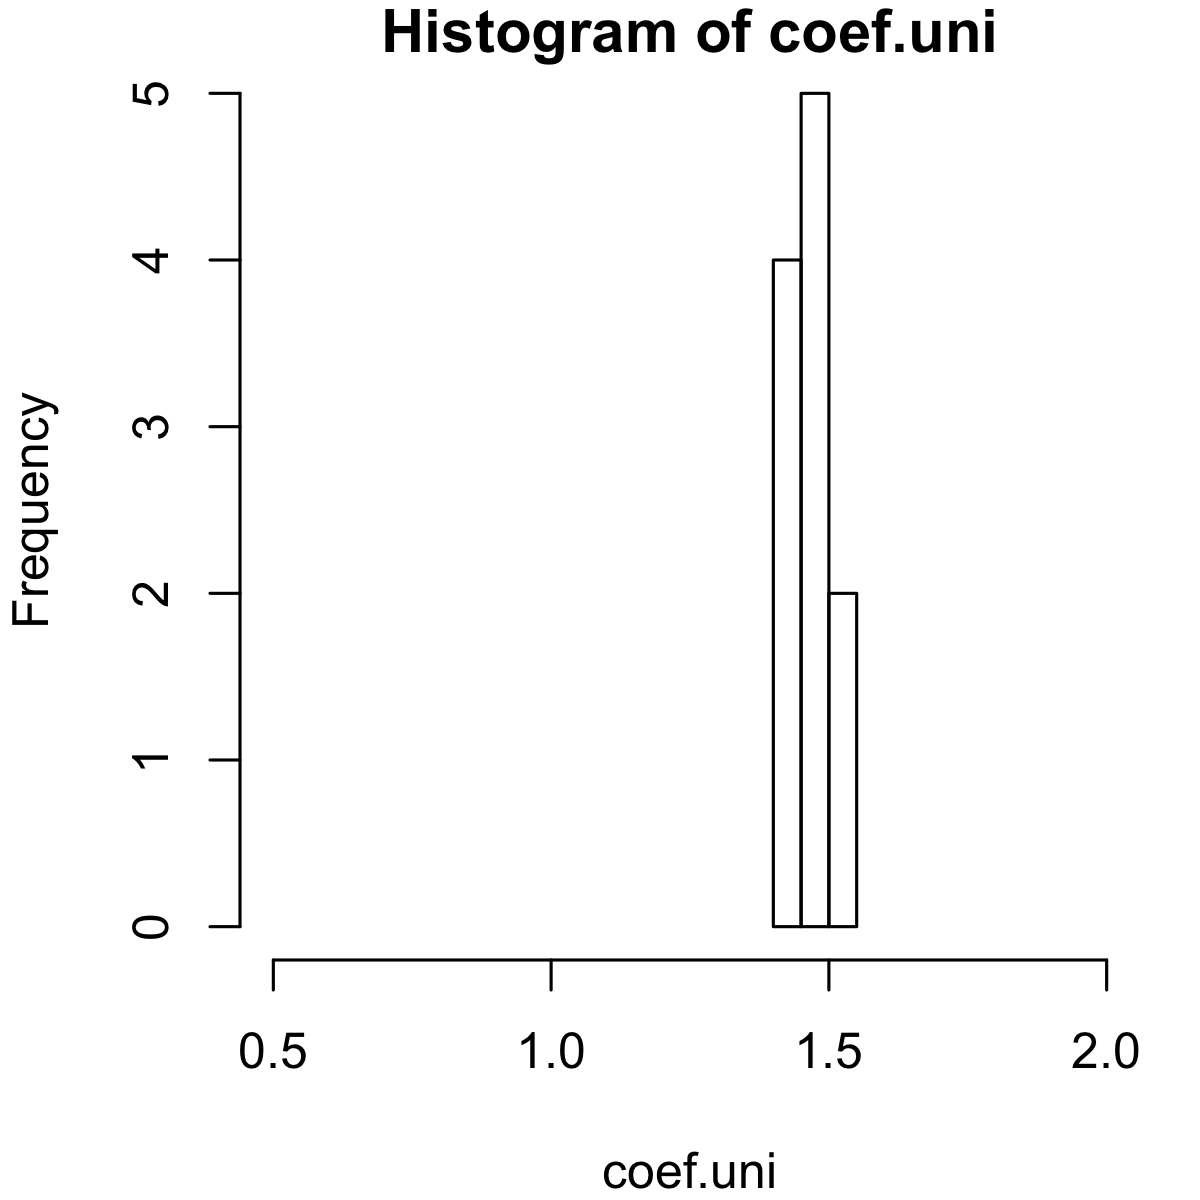
\includegraphics[width=0.48\textwidth]{img/coef-uni.png}
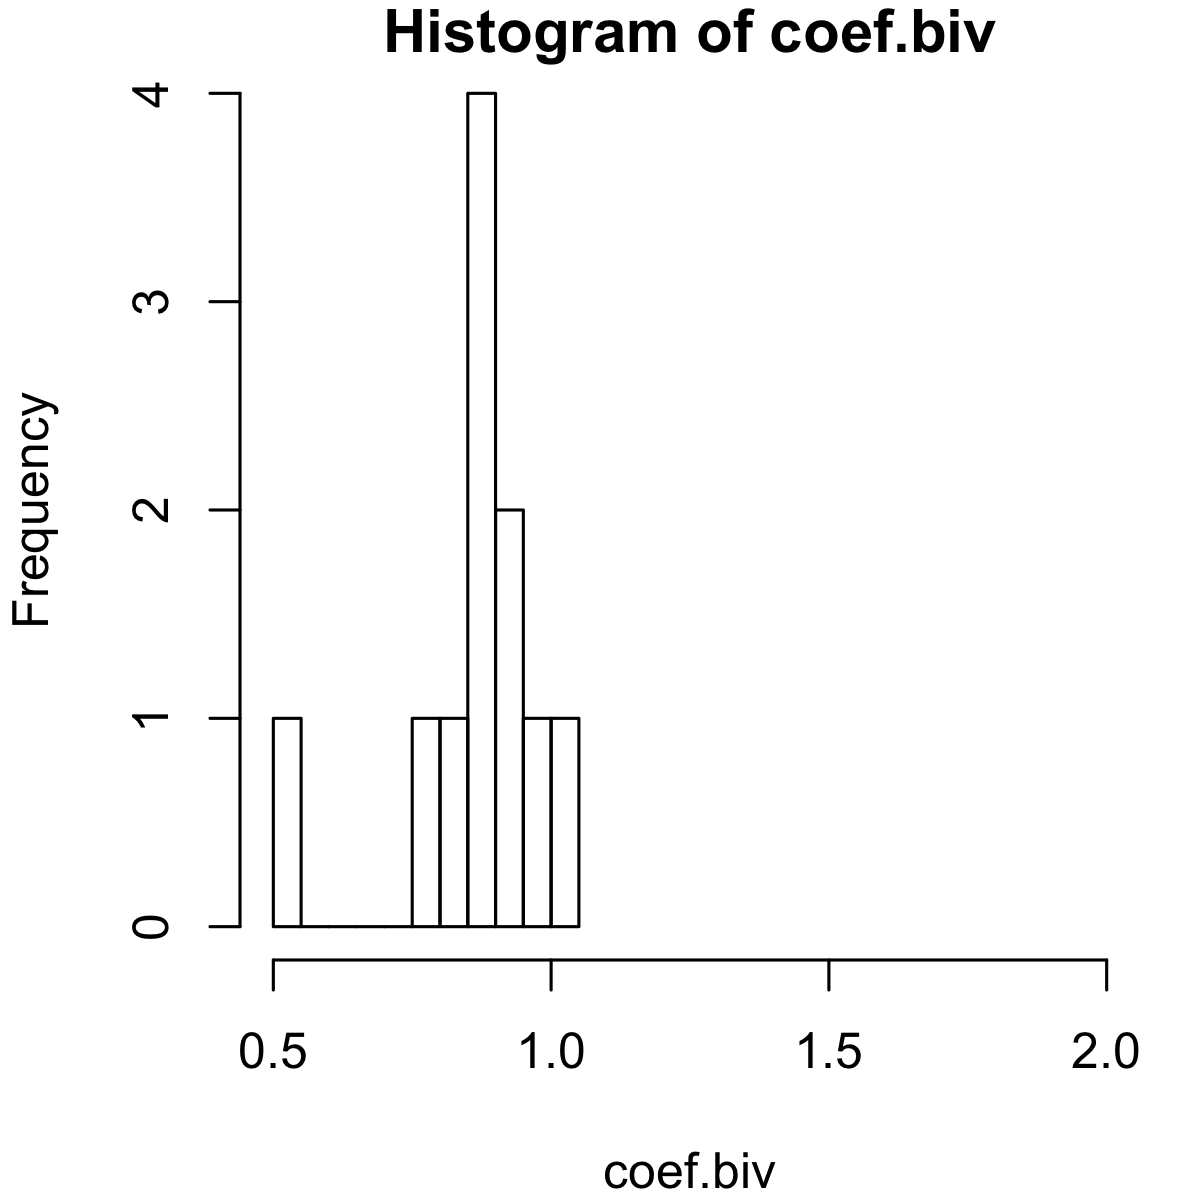
\includegraphics[width=0.48\textwidth]{img/coef-biv.png}
\end{center}

\paragraph{Question 16} Why is this bad?

\vspace{25mm}

\paragraph{What to Google:} Regularized/penalized regression; Lasso; Ridge regression; PCA and other matrix factorization techniques; variance inflation factor (try to regress each predictor on the others and calculate $R^2$ for these models)

\newpage

%%%%%%%%%%%%%%%%%%%%%%%%%%%%%%%%%%%%%%%%%%%%%%%%%%%%%%%%%%%%%%%%%%%%%%%%%%%%%%%%

\section{Non-Normality of Errors}

Only linear regression models assume normality of errors. Linear regression models are also typically quite robust to violations in the assumption that the errors are normally distributed. The coefficients themselves may be fine. However, hypothesis tests on the coefficients rely on the assumption of normality. So do confidence intervals on predictions (which rely on the standard errors of the coefficients). 

If the normality assumption is not true, it can lead to coefficients that look significant when they are not (or vice versa). It can also lead to prediction intervals that are artificially too wide or too narrow. 

Here are \textbf{QQ-plots} ({\color{blue} http://www.statisticshowto.com/q-q-plots/}) for the Anscombe's quartet example: \\[-10mm]
\begin{center}

\includegraphics[width=0.8\textwidth]{img/anscombe-diagnostics-2.png}
\end{center}
\vspace{-8mm}
\paragraph{What to Google:}
\begin{itemize}
\item Normality tests: {\color{blue} https://en.wikipedia.org/wiki/Normality\_test}
\item Some specific names: Kolmogorov-Smirnov, Shapiro-Wilk, Jarque-Bera, Anderson-Darling. Note that these are often too picky for real data.
\end{itemize}

\newpage


%%%%%%%%%%%%%%%%%%%%%%%%%%%%%%%%%%%%%%%%%%%%%%%%%%%%%%%%%%%%%%%%%%%%%%%%%%%%%%%%

\section{Outliers, High Leverage Points, and Influential Points}

Sometimes one or more datapoints have an outsized influence on the final form of a regression model. It's important to identify these points and figure out what to do with them (if anything) and what they are saying about your data/model. 

\begin{center}
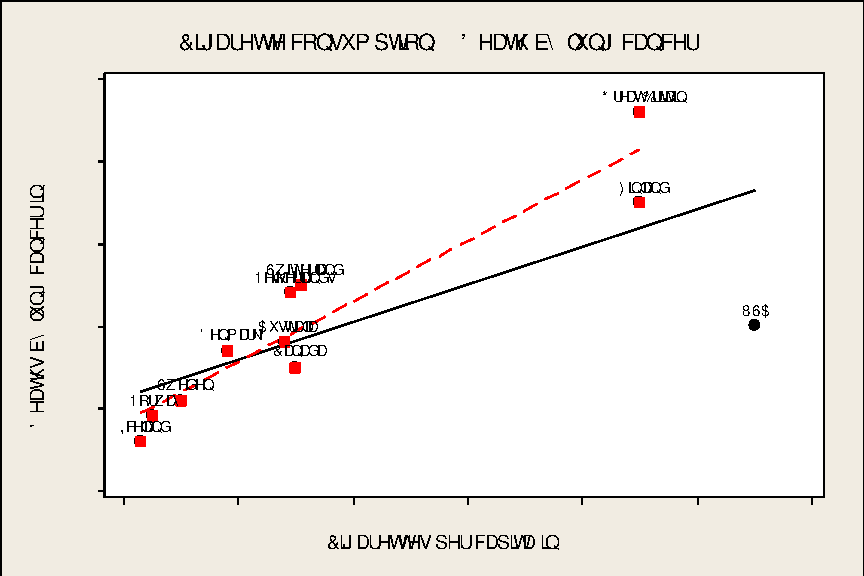
\includegraphics[width=0.65\textwidth]{img/cigarettes-lung-cancer.pdf}
\end{center}
{\small Source: Freedman et al 1991, as reproduced by Math 1530 professor at East Tennessee State University.}

\paragraph{Question 17} What is the difference between an \textbf{outlier} and a \textbf{high-leverage} point?

\vspace{30mm}

\paragraph{Question 18} What makes a point \textbf{influential}? Is the ``USA'' point an influential point in the plot above?

\newpage

\paragraph{Question 19} The following plots of Cook's distance (a measure of influence) are for the four plots in Anscombe's quartet. Do you detect any influential points in any of the plots? Be sure to take the $y$-axis scale into account. 
\begin{center}
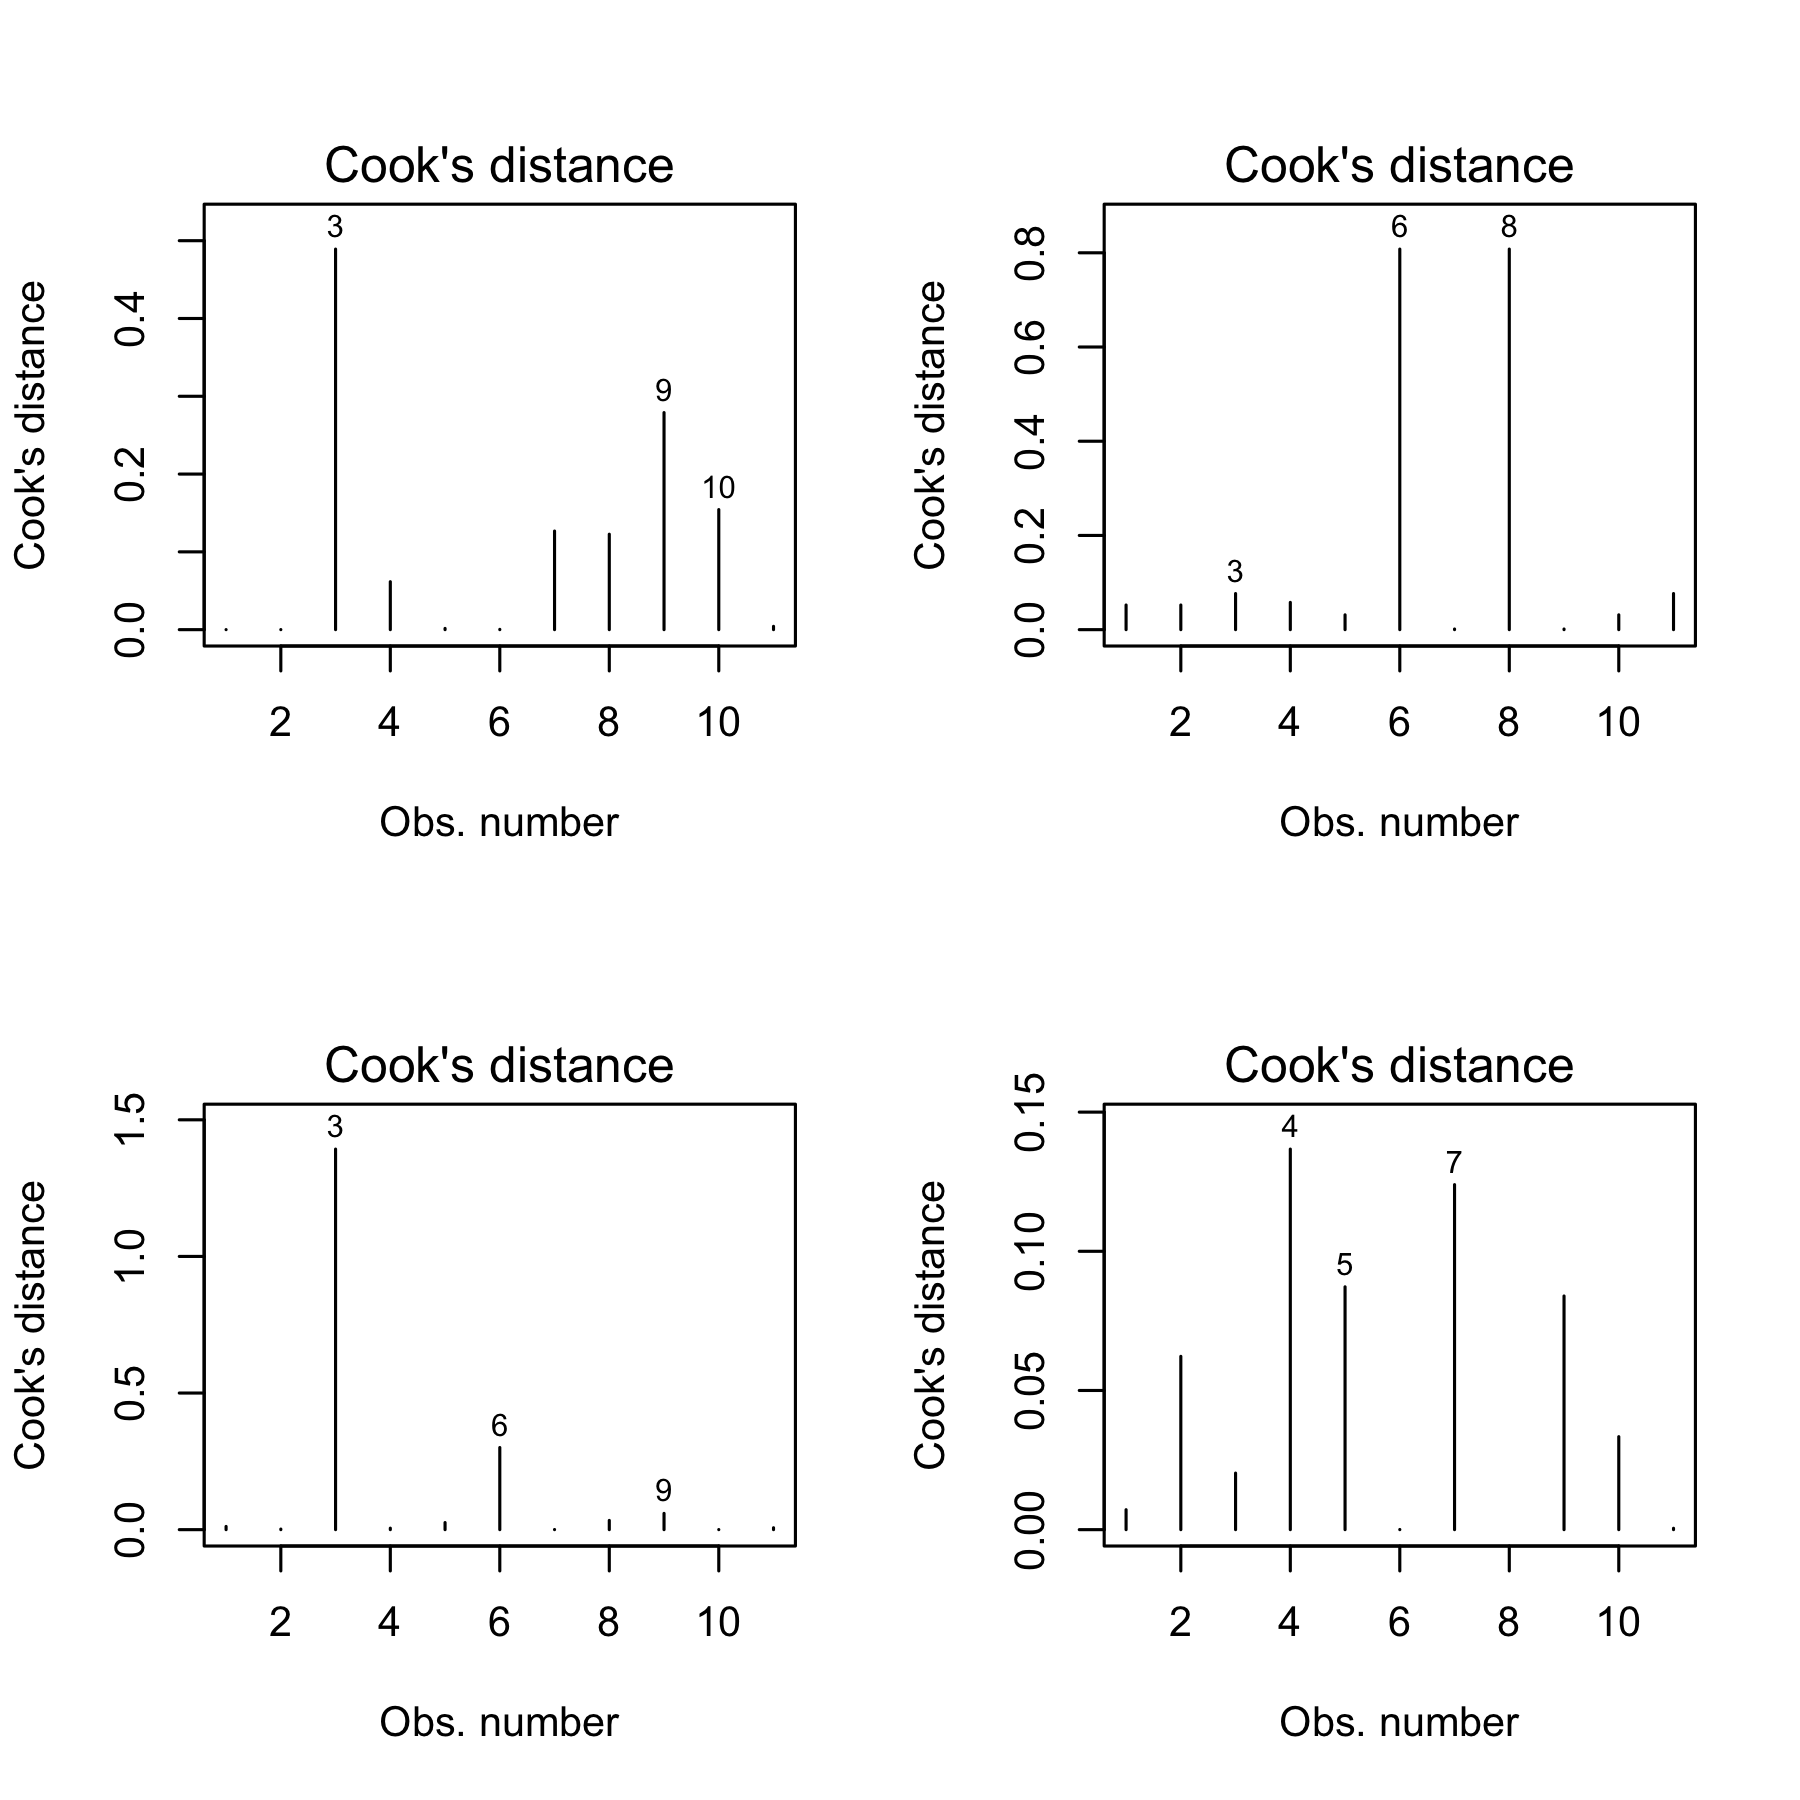
\includegraphics[width=0.8\textwidth]{img/anscombe-diagnostics-3.png}
\end{center}

\paragraph{What to Google:} Cook's distance, or Cook's D (a measure of how much model predictions change when a single observation is deleted); bagging

\newpage

%%%%%%%%%%%%%%%%%%%%%%%%%%%%%%%%%%%%%%%%%%%%%%%%%%%%%%%%%%%%%%%%%%%%%%%%%%%%%%%%

\section{Appendix: Generalized Linear Models}

\subsection{Modeling the Outcome}

\paragraph{Linear Regression} In linear regression, we assume that the outcome, $y$, is normal. Recall that the normal distribution is a continuous probability distribution with the following properties:

$$ p(y | \mu, \sigma) = \frac{1}{\sqrt{2 \pi \sigma^2}} e^{-\frac{(y-\mu)^2}{2 \sigma^2}} \qquad  E[y| \mu, \sigma] = \mu \qquad \text{var}(y | \mu, \sigma) = \sigma^2 $$

where $y \in \mathbb{R}$.

\paragraph{Logistic Regression} Logistic regression is used in cases where the outcome is binary: where $y$ is ``yes'' or ``no''. Variants of logistic regression, called \textbf{multinomial logistic regression} and the \textbf{proportional odds model}, can also be used to model data where the outcome contains multiple categories that either have an ordering (ordinal) or do not (nominal). 

In logistic regression, we assume that the outcome, $y$, is either $0$ or $1$. We model it using the Bernoulli distribution, which is a discrete probability distribution with the following properties:

$$ p(y|\mu) = \mu^y (1 - \mu) ^ {1-y} \qquad E[y| \mu] = \mu \qquad \text{var}(y | \mu) = \mu (1 - \mu) $$
where $y \in \{0, 1\}$.

\subsection{Modeling the Predictors}

All regression models incorporate a \textbf{linear combination} of predictors. A linear combination is an expression constructed from a set of terms by multiplying each term by a constant and adding the results.

We denote the number of predictors in the model by $p$, and denote the vector of predictors by $x$, where

$$ x = \begin{pmatrix}
1 \\
           x_{1} \\
           x_{2} \\
           \vdots \\
           x_{p}
         \end{pmatrix} $$
         
and we have included a ``1'' as the first element to allow for an \textbf{intercept}. We write $x^{(i)}$ to denote the vector of predictors associated with the $i$th training example.

The coefficients of the linear combination (i.e. the model parameters we are hoping to learn) are denoted by:

$$ \beta = \begin{pmatrix}
\beta_0 \\
           \beta_{1} \\
           \beta_{2} \\
           \vdots \\
           \beta_{p}
         \end{pmatrix} $$

and we often express the linear combination as an inner product, written as:

$$ \beta^T x = \beta_0 + \sum_{j=1}^p \beta_j x_j. $$

\subsection{Linking Predictors to Outcome}

All of the models we see today model the \textbf{expected value} of the outcome, $E[y]$ as some function of this linear combination of predictors. The function that relates the two is called the \textbf{link function}. Different types of regression use different link functions.

\paragraph{Linear Regression} In linear regression, the mean of the outcome distribution, which is normal, can be any real number. We therefore use the \textbf{identity link}, setting $E[y]$ directly equal to the linear combination of predictors. Since the outcome is normal, we know that $E[y] = \mu$, the mean of the normal distribution. We therefore write:

$$ E[y] = \mu = \beta^T x $$

which is usually rearranged and rewritten as:

$$ y = \beta^T x + \varepsilon $$

where $\varepsilon \sim N(0, \sigma^2)$. The relationship between $E[y]$ and $\beta^T x$ is shown in Figure~\ref{fig:identitylink}.

\begin{figure}
\begin{center}
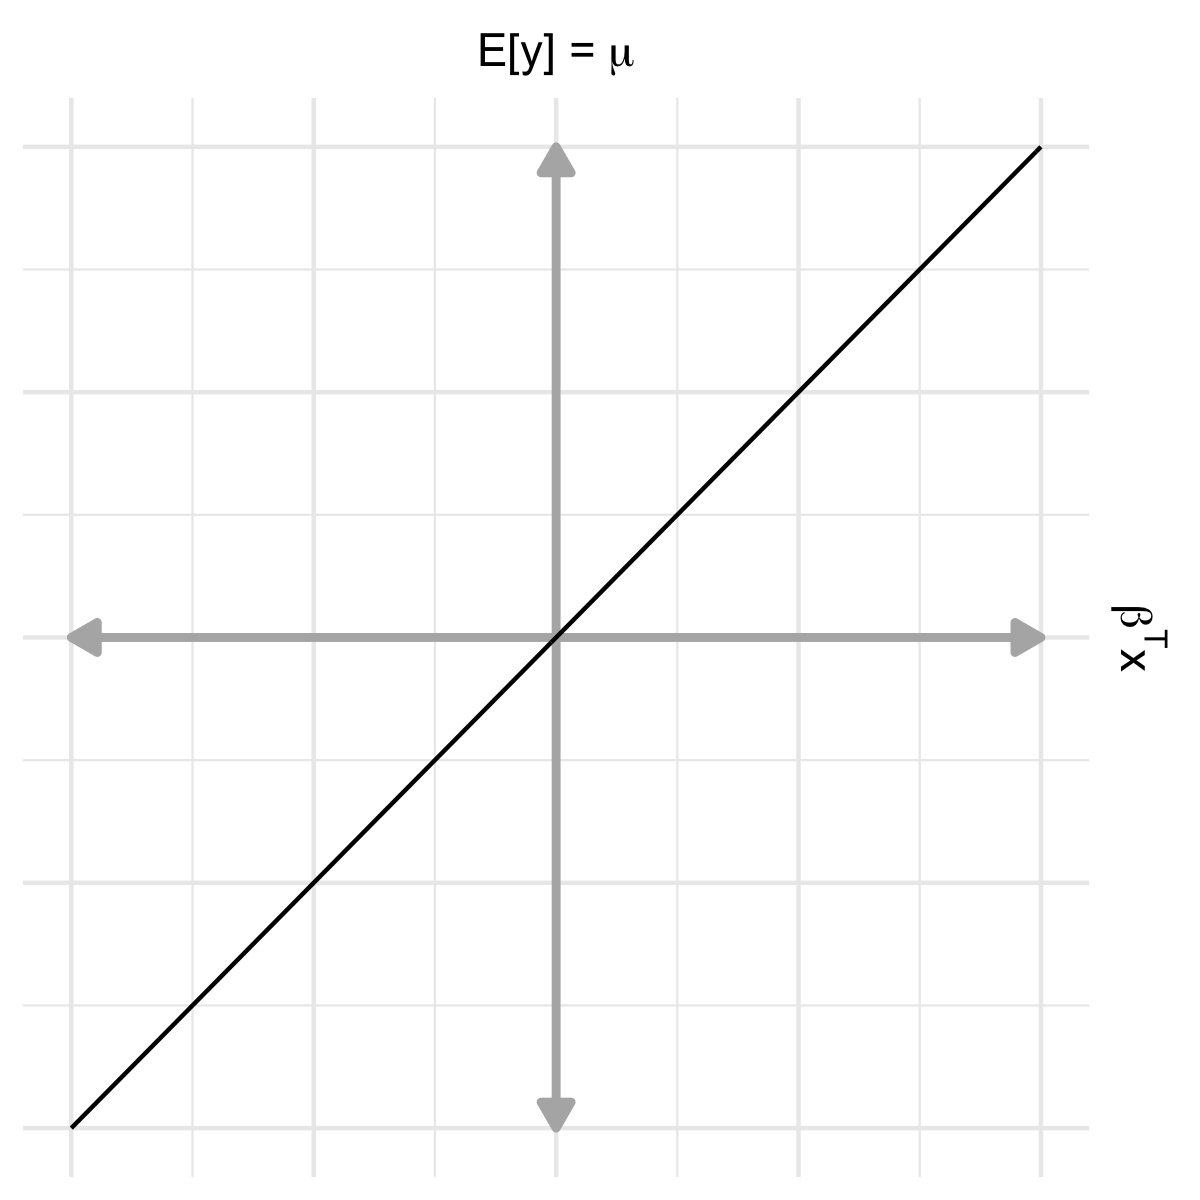
\includegraphics[width=3in]{img/l02-figure1-linreg.png}
\caption{The relationship between $E[y]$ and $\beta^T x$ in the linear regression model. \label{fig:identitylink}}
\end{center}
\end{figure}

\paragraph{Logistic Regression} In logistic regression, the mean of the outcome distribution, which is Bernoulli, is a probability. It must therefore be a real number between 0 and 1. No matter how large or small $\beta^T x$ gets, the value of $E[y] = \mu$ cannot be outside this range. We therefore apply the \textbf{logistic function}, $f(x) = 1/(1 + \exp(-x))$, which has the range $(0, 1)$, to $\beta^T x$ to squash it:

$$ E[y] = \mu = \frac{1}{1 + \exp{(-\beta^Tx)}} $$

The relationship between $E[y]$ and $\beta^T x$ is shown in Figure~\ref{fig:logitlink}.

\begin{figure}
\begin{center}
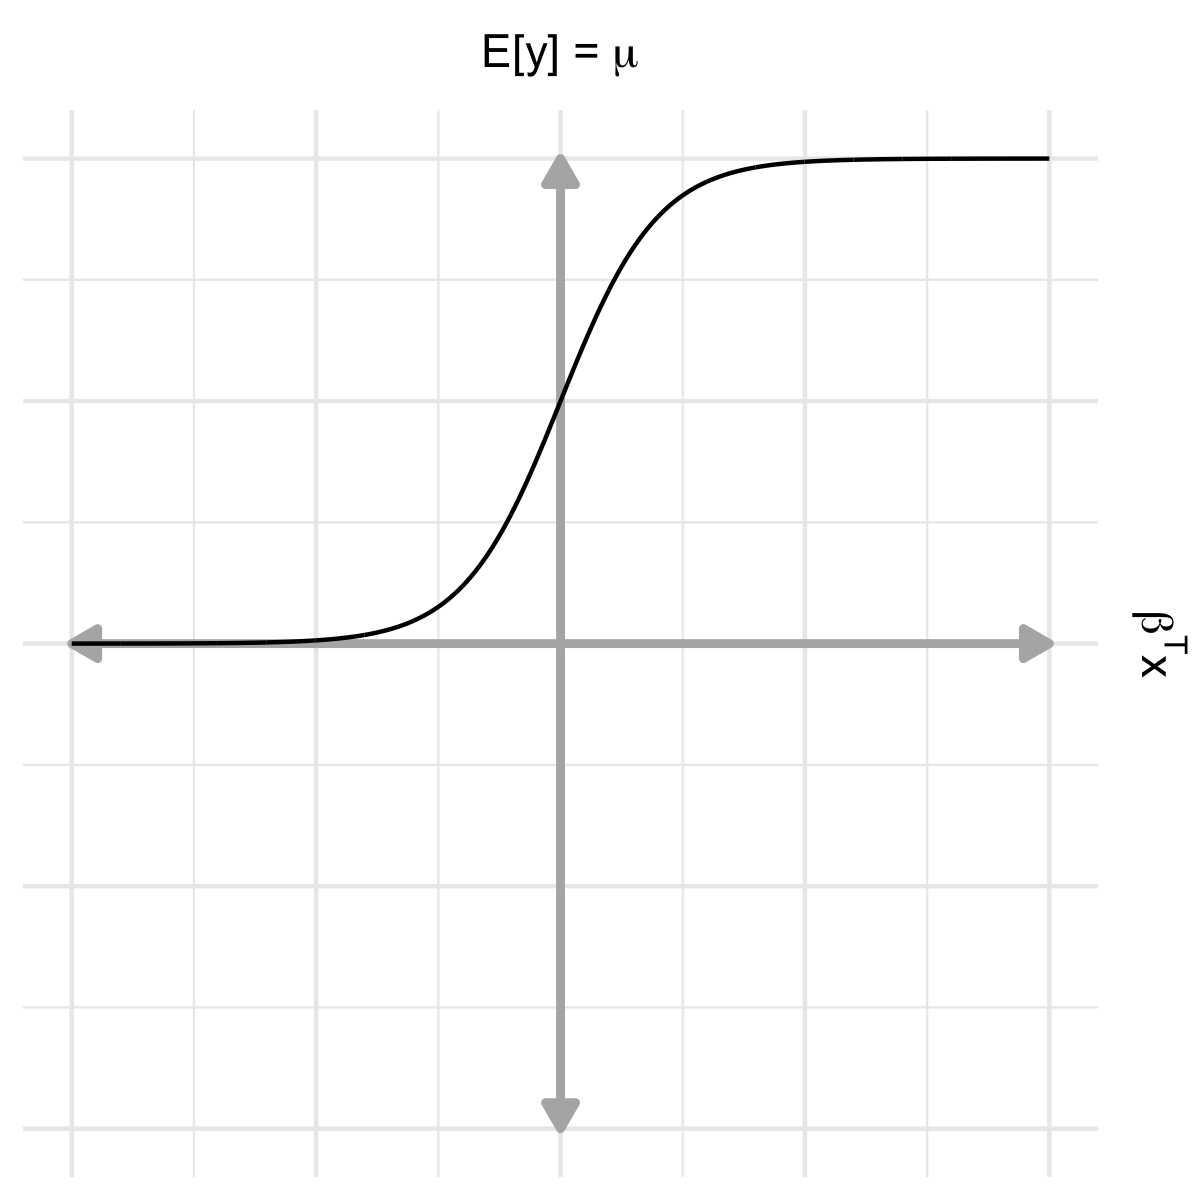
\includegraphics[width=3in]{img/l02-figure2-logistic.png}
\caption{The relationship between $E[y]$ and $\beta^T x$ in the logistic regression model. \label{fig:logitlink}}
\end{center}
\end{figure}

We typically invert the model to write

$$ \log{\frac{\mu}{1-\mu}} = \beta^T x $$

which is the standard form of the logistic regression model. The function $\log \left( \mu/(1-\mu) \right)$ is called the logit, and in logistic regression we say we use the \textbf{logit link}.

\newpage

%%%%%%%%%%%%%%%%%%%%%%%%%%%%%%%%%%%%%%%%%%%%%%%%%%%%%%%%%%%%%%%%%%%%%%%%%%%%%%%%

